\documentclass[twoside]{book}

% Packages required by doxygen
\usepackage{fixltx2e}
\usepackage{calc}
\usepackage{doxygen}
\usepackage{graphicx}
\usepackage[utf8]{inputenc}
\usepackage{makeidx}
\usepackage{multicol}
\usepackage{multirow}
\PassOptionsToPackage{warn}{textcomp}
\usepackage{textcomp}
\usepackage[nointegrals]{wasysym}
\usepackage[table]{xcolor}
\usepackage{ifpdf,ifxetex}

% Font selection
\usepackage[T1]{fontenc}
\usepackage[scaled=.90]{helvet}
\usepackage{courier}
\usepackage{amssymb}
\usepackage{sectsty}
\renewcommand{\familydefault}{\sfdefault}
\allsectionsfont{%
  \fontseries{bc}\selectfont%
  \color{darkgray}%
}
\renewcommand{\DoxyLabelFont}{%
  \fontseries{bc}\selectfont%
  \color{darkgray}%
}
\newcommand{\+}{\discretionary{\mbox{\scriptsize$\hookleftarrow$}}{}{}}

% Page & text layout
\usepackage{geometry}
\geometry{%
  a4paper,%
  top=2.5cm,%
  bottom=2.5cm,%
  left=2.5cm,%
  right=2.5cm%
}
\tolerance=750
\hfuzz=15pt
\hbadness=750
\setlength{\emergencystretch}{15pt}
\setlength{\parindent}{0cm}
\setlength{\parskip}{3ex plus 2ex minus 2ex}
\makeatletter
\renewcommand{\paragraph}{%
  \@startsection{paragraph}{4}{0ex}{-1.0ex}{1.0ex}{%
    \normalfont\normalsize\bfseries\SS@parafont%
  }%
}
\renewcommand{\subparagraph}{%
  \@startsection{subparagraph}{5}{0ex}{-1.0ex}{1.0ex}{%
    \normalfont\normalsize\bfseries\SS@subparafont%
  }%
}
\makeatother

% Headers & footers
\usepackage{fancyhdr}
\pagestyle{fancyplain}
\fancyhead[LE]{\fancyplain{}{\bfseries\thepage}}
\fancyhead[CE]{\fancyplain{}{}}
\fancyhead[RE]{\fancyplain{}{\bfseries\leftmark}}
\fancyhead[LO]{\fancyplain{}{\bfseries\rightmark}}
\fancyhead[CO]{\fancyplain{}{}}
\fancyhead[RO]{\fancyplain{}{\bfseries\thepage}}
\fancyfoot[LE]{\fancyplain{}{}}
\fancyfoot[CE]{\fancyplain{}{}}
\fancyfoot[RE]{\fancyplain{}{\bfseries\scriptsize Generated by Doxygen }}
\fancyfoot[LO]{\fancyplain{}{\bfseries\scriptsize Generated by Doxygen }}
\fancyfoot[CO]{\fancyplain{}{}}
\fancyfoot[RO]{\fancyplain{}{}}
\renewcommand{\footrulewidth}{0.4pt}
\renewcommand{\chaptermark}[1]{%
  \markboth{#1}{}%
}
\renewcommand{\sectionmark}[1]{%
  \markright{\thesection\ #1}%
}

% Indices & bibliography
\usepackage{natbib}
\usepackage[titles]{tocloft}
\setcounter{tocdepth}{3}
\setcounter{secnumdepth}{5}
\makeindex

% Hyperlinks (required, but should be loaded last)
\ifpdf
  \usepackage[pdftex,pagebackref=true]{hyperref}
\else
  \ifxetex
    \usepackage[pagebackref=true]{hyperref}
  \else
    \usepackage[ps2pdf,pagebackref=true]{hyperref}
  \fi
\fi
\ifpdf
  \DeclareUnicodeCharacter{207B}{${}^{-}$}% Superscript minus
  \DeclareUnicodeCharacter{C2B2}{${}^{2}$}% Superscript two
  \DeclareUnicodeCharacter{C2B3}{${}^{3}$}% Superscript three
\else
  \catcode`\⁻=13% Superscript minus
  \def⁻{${}^{-}$}
  \catcode`\²=13% Superscript two
  \def²{${}^{2}$}
  \catcode`\³=13% Superscript three
  \def³{${}^{3}$}
\fi

\hypersetup{%
  colorlinks=true,%
  linkcolor=blue,%
  citecolor=blue,%
  unicode%
}

% Custom commands
\newcommand{\clearemptydoublepage}{%
  \newpage{\pagestyle{empty}\cleardoublepage}%
}

\usepackage{caption}
\captionsetup{labelsep=space,justification=centering,font={bf},singlelinecheck=off,skip=4pt,position=top}

\renewcommand{\numberline}[1]{#1~}
%===== C O N T E N T S =====

\begin{document}

% Titlepage & ToC
\hypersetup{pageanchor=false,
             bookmarksnumbered=true,
             pdfencoding=unicode
            }
\pagenumbering{alph}
\begin{titlepage}
\vspace*{7cm}
\begin{center}%
{\Large Projet C\+IR2 }\\
\vspace*{1cm}
{\large Generated by Doxygen 1.8.15}\\
\end{center}
\end{titlepage}
\clearemptydoublepage
\pagenumbering{roman}
\tableofcontents
\clearemptydoublepage
\pagenumbering{arabic}
\hypersetup{pageanchor=true}

%--- Begin generated contents ---
\chapter{Hierarchical Index}
\section{Class Hierarchy}
This inheritance list is sorted roughly, but not completely, alphabetically\+:\begin{DoxyCompactList}
\item \contentsline{section}{Database}{\pageref{classDatabase}}{}
\item \contentsline{section}{MD5}{\pageref{classMD5}}{}
\item \contentsline{section}{Proposition}{\pageref{classProposition}}{}
\item Q\+Main\+Window\begin{DoxyCompactList}
\item \contentsline{section}{Main\+Window}{\pageref{classMainWindow}}{}
\item \contentsline{section}{Manage\+Window}{\pageref{classManageWindow}}{}
\end{DoxyCompactList}
\item \contentsline{section}{Question}{\pageref{classQuestion}}{}
\item \contentsline{section}{Theme}{\pageref{classTheme}}{}
\item \contentsline{section}{Themes}{\pageref{classThemes}}{}
\item \contentsline{section}{User}{\pageref{classUser}}{}
\end{DoxyCompactList}

\chapter{Class Index}
\section{Class List}
Here are the classes, structs, unions and interfaces with brief descriptions\+:\begin{DoxyCompactList}
\item\contentsline{section}{\mbox{\hyperlink{classDatabase}{Database}} \\*Classe de la base de donnée }{\pageref{classDatabase}}{}
\item\contentsline{section}{\mbox{\hyperlink{classMainWindow}{Main\+Window}} \\*Une classe Qt pour gerer la fenetre de connexion }{\pageref{classMainWindow}}{}
\item\contentsline{section}{\mbox{\hyperlink{classManageWindow}{Manage\+Window}} \\*Une classe Qt pour gerer la fenetre de gestion de la B\+DD }{\pageref{classManageWindow}}{}
\item\contentsline{section}{\mbox{\hyperlink{classMD5}{M\+D5}} \\*Small class for calculating \mbox{\hyperlink{classMD5}{M\+D5}} hashes of strings or byte arrays it is not meant to be fast or secure }{\pageref{classMD5}}{}
\item\contentsline{section}{\mbox{\hyperlink{classProposition}{Proposition}} \\*Une classe C++ pour stocker une proposition recuperee en B\+DD }{\pageref{classProposition}}{}
\item\contentsline{section}{\mbox{\hyperlink{classQuestion}{Question}} \\*Une classe C++ pour stocker une question recuperee en B\+DD }{\pageref{classQuestion}}{}
\item\contentsline{section}{\mbox{\hyperlink{classTheme}{Theme}} }{\pageref{classTheme}}{}
\item\contentsline{section}{\mbox{\hyperlink{classThemes}{Themes}} \\*Une classe C++ pour stocker un theme recupéré en B\+DD }{\pageref{classThemes}}{}
\item\contentsline{section}{\mbox{\hyperlink{classUser}{User}} }{\pageref{classUser}}{}
\end{DoxyCompactList}

\chapter{File Index}
\section{File List}
Here is a list of all documented files with brief descriptions\+:\begin{DoxyCompactList}
\item\contentsline{section}{Headers/\mbox{\hyperlink{database_8hpp}{database.\+hpp}} \\*Fichier contenant la classe \mbox{\hyperlink{classDatabase}{Database}} }{\pageref{database_8hpp}}{}
\item\contentsline{section}{Headers/\mbox{\hyperlink{includes_8hpp}{includes.\+hpp}} \\*Fichier contenant tous les include necessaires }{\pageref{includes_8hpp}}{}
\item\contentsline{section}{Headers/\mbox{\hyperlink{mainwindow_8hpp}{mainwindow.\+hpp}} \\*Fichier contenant la classe \mbox{\hyperlink{classMainWindow}{Main\+Window}} }{\pageref{mainwindow_8hpp}}{}
\item\contentsline{section}{Headers/\mbox{\hyperlink{managewindow_8hpp}{managewindow.\+hpp}} \\*Fichier contenant la classe \mbox{\hyperlink{classManageWindow}{Manage\+Window}} }{\pageref{managewindow_8hpp}}{}
\item\contentsline{section}{Headers/\mbox{\hyperlink{md5_8hpp}{md5.\+hpp}} \\*Fichier contenant la classe \mbox{\hyperlink{classMD5}{M\+D5}} }{\pageref{md5_8hpp}}{}
\item\contentsline{section}{Headers/\mbox{\hyperlink{proposition_8hpp}{proposition.\+hpp}} \\*Fichier contenant la classe \mbox{\hyperlink{classProposition}{Proposition}} }{\pageref{proposition_8hpp}}{}
\item\contentsline{section}{Headers/\mbox{\hyperlink{question_8hpp}{question.\+hpp}} \\*Fichier contenant la classe \mbox{\hyperlink{classQuestion}{Question}} }{\pageref{question_8hpp}}{}
\item\contentsline{section}{Headers/\mbox{\hyperlink{theme_8hpp}{theme.\+hpp}} \\*Fichier contenant la classe \mbox{\hyperlink{classTheme}{Theme}} }{\pageref{theme_8hpp}}{}
\item\contentsline{section}{Headers/\mbox{\hyperlink{user_8hpp}{user.\+hpp}} \\*Fichier contenant la classe \mbox{\hyperlink{classUser}{User}} }{\pageref{user_8hpp}}{}
\item\contentsline{section}{Sources/\mbox{\hyperlink{database_8cpp}{database.\+cpp}} \\*Fichier contenant les methodes de la classe \mbox{\hyperlink{classDatabase}{Database}} }{\pageref{database_8cpp}}{}
\item\contentsline{section}{Sources/\mbox{\hyperlink{main_8cpp}{main.\+cpp}} \\*Fichier principal de l\textquotesingle{}application }{\pageref{main_8cpp}}{}
\item\contentsline{section}{Sources/\mbox{\hyperlink{mainwindow_8cpp}{mainwindow.\+cpp}} \\*Fichier contenant les methodes de la classe \mbox{\hyperlink{classMainWindow}{Main\+Window}} }{\pageref{mainwindow_8cpp}}{}
\item\contentsline{section}{Sources/\mbox{\hyperlink{managewindow_8cpp}{managewindow.\+cpp}} \\*Fichier contenant les methodes de la classe \mbox{\hyperlink{classManageWindow}{Manage\+Window}} }{\pageref{managewindow_8cpp}}{}
\item\contentsline{section}{Sources/\mbox{\hyperlink{proposition_8cpp}{proposition.\+cpp}} \\*Fichier contenant les methodes de la classe \mbox{\hyperlink{classProposition}{Proposition}} }{\pageref{proposition_8cpp}}{}
\item\contentsline{section}{Sources/\mbox{\hyperlink{question_8cpp}{question.\+cpp}} \\*Fichier contenant les methodes de la classe \mbox{\hyperlink{classQuestion}{Question}} }{\pageref{question_8cpp}}{}
\item\contentsline{section}{Sources/\mbox{\hyperlink{theme_8cpp}{theme.\+cpp}} \\*Fichier contenant les methodes de la classe \mbox{\hyperlink{classTheme}{Theme}} }{\pageref{theme_8cpp}}{}
\item\contentsline{section}{Sources/\mbox{\hyperlink{user_8cpp}{user.\+cpp}} \\*Fichier contenant les methodes de la classe \mbox{\hyperlink{classUser}{User}} }{\pageref{user_8cpp}}{}
\end{DoxyCompactList}

\chapter{Class Documentation}
\hypertarget{classDatabase}{}\section{Database Class Reference}
\label{classDatabase}\index{Database@{Database}}


Classe de la base de donnée.  




{\ttfamily \#include $<$database.\+hpp$>$}

\subsection*{Public Member Functions}
\begin{DoxyCompactItemize}
\item 
\mbox{\hyperlink{classDatabase_a95206f04bf344b042799c9bed2bc29ad}{Database}} (string ip\+Address, string db\+Name, string db\+Pwd)
\begin{DoxyCompactList}\small\item\em Constructeur. \end{DoxyCompactList}\item 
\mbox{\hyperlink{classDatabase_a84d399a2ad58d69daab9b05330e1316d}{$\sim$\+Database}} ()
\begin{DoxyCompactList}\small\item\em Destructeur. \end{DoxyCompactList}\item 
string \mbox{\hyperlink{classDatabase_aa3d736693ce3f873f29078c89c57df93}{check\+Apostrophes}} (string statement)
\begin{DoxyCompactList}\small\item\em Verification de syntaxe. \end{DoxyCompactList}\item 
bool \mbox{\hyperlink{classDatabase_aab00e57287fe5e19c727c6cd2cadc154}{test\+Admin}} (string user, string pwd)
\begin{DoxyCompactList}\small\item\em Verification de syntaxe. \end{DoxyCompactList}\item 
bool \mbox{\hyperlink{classDatabase_adbff1128a3de654905631045f56955f0}{check\+If\+Exists}} (string table, string row, string token)
\begin{DoxyCompactList}\small\item\em Fonction de test. \end{DoxyCompactList}\item 
void \mbox{\hyperlink{classDatabase_a725966780835e8a3c1315fbdce50258f}{list\+Themes}} ()
\begin{DoxyCompactList}\small\item\em Fonction de récupération de données. \end{DoxyCompactList}\item 
void \mbox{\hyperlink{classDatabase_ae5bacbdc2d6804c63d79cdafc249dd64}{list\+Questions\+\_\+order\+\_\+by\+\_\+\+Categorie}} ()
\begin{DoxyCompactList}\small\item\em Fonction de récupération de données. \end{DoxyCompactList}\item 
void \mbox{\hyperlink{classDatabase_a184cd88b6dfcc3938b699107b693d642}{list\+Propositions}} (int id\+\_\+question)
\begin{DoxyCompactList}\small\item\em Fonction de récupération de données. \end{DoxyCompactList}\item 
void \mbox{\hyperlink{classDatabase_adf142a6306d28877edca6de39a4b7bc1}{list\+Users}} ()
\begin{DoxyCompactList}\small\item\em Fonction de récupération de données. \end{DoxyCompactList}\item 
int \mbox{\hyperlink{classDatabase_a4b452a64336f21e9ff02495c6f52b0fc}{get\+Id}} (string id, string table, string row, string token)
\begin{DoxyCompactList}\small\item\em Fonction de récupération de données. \end{DoxyCompactList}\item 
string \mbox{\hyperlink{classDatabase_aa521990114ae753ab5cea9b7ebf3ca01}{get\+Pwd}} (string user)
\begin{DoxyCompactList}\small\item\em Fonction de récupération de données. \end{DoxyCompactList}\item 
void \mbox{\hyperlink{classDatabase_a15faf1f7341da9efee62afacd31fb81d}{add\+Theme}} (string new\+Name)
\begin{DoxyCompactList}\small\item\em Fonction d\textquotesingle{}ajout de donnees. \end{DoxyCompactList}\item 
void \mbox{\hyperlink{classDatabase_afcefe4bac17bcc073c8f14679c375a35}{add\+Question}} (string new\+Question, int id\+Theme)
\begin{DoxyCompactList}\small\item\em Fonction d\textquotesingle{}ajout de donnees. \end{DoxyCompactList}\item 
void \mbox{\hyperlink{classDatabase_adb9d2a51e963cf93bcfc0c47ce2e1d72}{add\+Prop}} (string proposition, int good\+Answer, int id\+Question)
\begin{DoxyCompactList}\small\item\em Fonction d\textquotesingle{}ajout de donnees. \end{DoxyCompactList}\item 
void \mbox{\hyperlink{classDatabase_a5e69b420a56127d86aca142683e03cbf}{add\+User}} (string username, string password, int check\+Admin)
\begin{DoxyCompactList}\small\item\em Fonction d\textquotesingle{}ajout de donnees. \end{DoxyCompactList}\item 
void \mbox{\hyperlink{classDatabase_a88ac52b22562c45d1e54610ee5ac4026}{edit\+Theme}} (string theme, string new\+Name)
\begin{DoxyCompactList}\small\item\em Fonction d\textquotesingle{}edition de donnees. \end{DoxyCompactList}\item 
void \mbox{\hyperlink{classDatabase_ac402414daf1786c1a9189fe29c18e345}{edit\+Question}} (string new\+Question, int id\+\_\+question)
\begin{DoxyCompactList}\small\item\em Fonction d\textquotesingle{}edition de donnees. \end{DoxyCompactList}\item 
void \mbox{\hyperlink{classDatabase_a63fefba403dae2942256ee1704ee282a}{edit\+Prop}} (string proposition, int good\+Answer, int id\+\_\+question, int id\+\_\+proposition)
\begin{DoxyCompactList}\small\item\em Fonction d\textquotesingle{}edition de donnees. \end{DoxyCompactList}\item 
void \mbox{\hyperlink{classDatabase_a2c742ca4a931b676f099951fe9dea256}{edit\+User}} (string user, string new\+Name, string new\+Pwd, int check\+Admin)
\begin{DoxyCompactList}\small\item\em Fonction d\textquotesingle{}edition de donnees. \end{DoxyCompactList}\item 
void \mbox{\hyperlink{classDatabase_a1b99f71f520f57eb4dc53e7ad709660e}{del\+Theme}} (int id\+\_\+ctg)
\begin{DoxyCompactList}\small\item\em Fonction de suppression de données. \end{DoxyCompactList}\item 
void \mbox{\hyperlink{classDatabase_a67a8d9eaa8a34e98606cf5233cbaa77f}{del\+Question}} (string question, int id\+\_\+question)
\begin{DoxyCompactList}\small\item\em Fonction de suppression de données. \end{DoxyCompactList}\item 
void \mbox{\hyperlink{classDatabase_a58ea1f635ec948e38bdbcfec9dd98a5e}{del\+Prop}} (string proposition)
\begin{DoxyCompactList}\small\item\em Fonction de suppression de données. \end{DoxyCompactList}\item 
void \mbox{\hyperlink{classDatabase_a6c40c150a977a2c4c4a1c01fe48e7c71}{del\+User}} (string username)
\begin{DoxyCompactList}\small\item\em Fonction de suppression de données. \end{DoxyCompactList}\item 
vector$<$ \mbox{\hyperlink{classTheme}{Theme}} $>$ \mbox{\hyperlink{classDatabase_a4cc8ad17cfd1cbf1074e56aa1e2eb71d}{get\+Themes}} ()
\begin{DoxyCompactList}\small\item\em Getter. \end{DoxyCompactList}\item 
vector$<$ \mbox{\hyperlink{classQuestion}{Question}} $>$ \mbox{\hyperlink{classDatabase_ae1aff982221c7ed188e1ce3ed00f878d}{get\+Questions}} ()
\begin{DoxyCompactList}\small\item\em Getter. \end{DoxyCompactList}\item 
vector$<$ \mbox{\hyperlink{classProposition}{Proposition}} $>$ \mbox{\hyperlink{classDatabase_a19e779ae9923798268d4b7052b09a76f}{get\+Propositions}} ()
\begin{DoxyCompactList}\small\item\em Getter. \end{DoxyCompactList}\item 
vector$<$ \mbox{\hyperlink{classUser}{User}} $>$ \mbox{\hyperlink{classDatabase_a78d088be3546d65b81e532d931a90f22}{get\+Users}} ()
\begin{DoxyCompactList}\small\item\em Getter. \end{DoxyCompactList}\end{DoxyCompactItemize}


\subsection{Detailed Description}
Classe de la base de donnée. 

La classe se connecte a la bdd et contient les fonctions effectuant les requetes S\+QL 

\subsection{Constructor \& Destructor Documentation}
\mbox{\Hypertarget{classDatabase_a95206f04bf344b042799c9bed2bc29ad}\label{classDatabase_a95206f04bf344b042799c9bed2bc29ad}} 
\index{Database@{Database}!Database@{Database}}
\index{Database@{Database}!Database@{Database}}
\subsubsection{\texorpdfstring{Database()}{Database()}}
{\footnotesize\ttfamily Database\+::\+Database (\begin{DoxyParamCaption}\item[{string}]{ip\+Address,  }\item[{string}]{db\+Name,  }\item[{string}]{db\+Pwd }\end{DoxyParamCaption})}



Constructeur. 

Constructeur de la classe \mbox{\hyperlink{classDatabase}{Database}}. Il recupere les drivers sql, se connecte a la B\+DD et initialise sql\+::\+Statement $\ast$stmt


\begin{DoxyParams}{Parameters}
{\em std\+::string} & ip\+Address \+: L\textquotesingle{}adresse ip de la B\+DD \\
\hline
{\em std\+::string} & db\+Name \+: Le nom de la B\+DD \\
\hline
{\em std\+::string} & db\+Pwd \+: Le mot de passe de la B\+DD \\
\hline
\end{DoxyParams}
\mbox{\Hypertarget{classDatabase_a84d399a2ad58d69daab9b05330e1316d}\label{classDatabase_a84d399a2ad58d69daab9b05330e1316d}} 
\index{Database@{Database}!````~Database@{$\sim$\+Database}}
\index{````~Database@{$\sim$\+Database}!Database@{Database}}
\subsubsection{\texorpdfstring{$\sim$\+Database()}{~Database()}}
{\footnotesize\ttfamily Database\+::$\sim$\+Database (\begin{DoxyParamCaption}{ }\end{DoxyParamCaption})}



Destructeur. 

Destructeur de la classe \mbox{\hyperlink{classDatabase}{Database}} 

\subsection{Member Function Documentation}
\mbox{\Hypertarget{classDatabase_adb9d2a51e963cf93bcfc0c47ce2e1d72}\label{classDatabase_adb9d2a51e963cf93bcfc0c47ce2e1d72}} 
\index{Database@{Database}!add\+Prop@{add\+Prop}}
\index{add\+Prop@{add\+Prop}!Database@{Database}}
\subsubsection{\texorpdfstring{add\+Prop()}{addProp()}}
{\footnotesize\ttfamily void Database\+::add\+Prop (\begin{DoxyParamCaption}\item[{string}]{proposition,  }\item[{int}]{good\+Answer,  }\item[{int}]{id\+Question }\end{DoxyParamCaption})}



Fonction d\textquotesingle{}ajout de donnees. 

Cette fonction permet d\textquotesingle{}ajouter une proposition 
\begin{DoxyParams}{Parameters}
{\em std\+::string} & proposition \+: Le nom de la nouvelle proposition \\
\hline
{\em int} & good\+Answer \+: La bonne reponse choisie (1,2 ou 3) \\
\hline
{\em int} & id\+Question \+: l\textquotesingle{}id de la question associée \\
\hline
\end{DoxyParams}
\mbox{\Hypertarget{classDatabase_afcefe4bac17bcc073c8f14679c375a35}\label{classDatabase_afcefe4bac17bcc073c8f14679c375a35}} 
\index{Database@{Database}!add\+Question@{add\+Question}}
\index{add\+Question@{add\+Question}!Database@{Database}}
\subsubsection{\texorpdfstring{add\+Question()}{addQuestion()}}
{\footnotesize\ttfamily void Database\+::add\+Question (\begin{DoxyParamCaption}\item[{string}]{new\+Question,  }\item[{int}]{id\+Theme }\end{DoxyParamCaption})}



Fonction d\textquotesingle{}ajout de donnees. 

Cette fonction permet d\textquotesingle{}ajouter une question 
\begin{DoxyParams}{Parameters}
{\em std\+::string} & new\+Question \+: Le nom de la nouvelle question \\
\hline
{\em int} & id\+Theme \+: L\textquotesingle{}id du theme de la nouvelle question \\
\hline
\end{DoxyParams}
\mbox{\Hypertarget{classDatabase_a15faf1f7341da9efee62afacd31fb81d}\label{classDatabase_a15faf1f7341da9efee62afacd31fb81d}} 
\index{Database@{Database}!add\+Theme@{add\+Theme}}
\index{add\+Theme@{add\+Theme}!Database@{Database}}
\subsubsection{\texorpdfstring{add\+Theme()}{addTheme()}}
{\footnotesize\ttfamily void Database\+::add\+Theme (\begin{DoxyParamCaption}\item[{string}]{new\+Name }\end{DoxyParamCaption})}



Fonction d\textquotesingle{}ajout de donnees. 

Cette fonction permet d\textquotesingle{}ajouter un theme 
\begin{DoxyParams}{Parameters}
{\em std\+::string} & new\+Name \+: Le nom du nouveau theme \\
\hline
\end{DoxyParams}
\mbox{\Hypertarget{classDatabase_a5e69b420a56127d86aca142683e03cbf}\label{classDatabase_a5e69b420a56127d86aca142683e03cbf}} 
\index{Database@{Database}!add\+User@{add\+User}}
\index{add\+User@{add\+User}!Database@{Database}}
\subsubsection{\texorpdfstring{add\+User()}{addUser()}}
{\footnotesize\ttfamily void Database\+::add\+User (\begin{DoxyParamCaption}\item[{string}]{username,  }\item[{string}]{password,  }\item[{int}]{check\+Admin }\end{DoxyParamCaption})}



Fonction d\textquotesingle{}ajout de donnees. 

Cette fonction permet d\textquotesingle{}ajouter un utilisateur 
\begin{DoxyParams}{Parameters}
{\em std\+::string} & username \+: Le nom de l\textquotesingle{}utilisateur \\
\hline
{\em std\+::string} & password \+: Le nouveau nom a donner a cet utilisateur \\
\hline
{\em int} & check\+Admin \+: Etat de la Q\+Check\+Box (0,1 ou 2) pour mettre l\textquotesingle{}utilisateur en admin ou non \\
\hline
\end{DoxyParams}
\mbox{\Hypertarget{classDatabase_aa3d736693ce3f873f29078c89c57df93}\label{classDatabase_aa3d736693ce3f873f29078c89c57df93}} 
\index{Database@{Database}!check\+Apostrophes@{check\+Apostrophes}}
\index{check\+Apostrophes@{check\+Apostrophes}!Database@{Database}}
\subsubsection{\texorpdfstring{check\+Apostrophes()}{checkApostrophes()}}
{\footnotesize\ttfamily string Database\+::check\+Apostrophes (\begin{DoxyParamCaption}\item[{string}]{statement }\end{DoxyParamCaption})}



Verification de syntaxe. 

Cette fonction renvoie la chaine entrée après avoir doublé les apostrophes s\textquotesingle{}il y en a. Les apostrophes sont sources d\textquotesingle{}erreurs dans les requetes S\+QL, on les double pour eviter ces problemes.


\begin{DoxyParams}{Parameters}
{\em std\+::string} & statement \+: La chaine a verifier \\
\hline
\end{DoxyParams}
\begin{DoxyReturn}{Returns}
std\+::string statement \+: La chaine verifiée 
\end{DoxyReturn}
\mbox{\Hypertarget{classDatabase_adbff1128a3de654905631045f56955f0}\label{classDatabase_adbff1128a3de654905631045f56955f0}} 
\index{Database@{Database}!check\+If\+Exists@{check\+If\+Exists}}
\index{check\+If\+Exists@{check\+If\+Exists}!Database@{Database}}
\subsubsection{\texorpdfstring{check\+If\+Exists()}{checkIfExists()}}
{\footnotesize\ttfamily bool Database\+::check\+If\+Exists (\begin{DoxyParamCaption}\item[{string}]{table,  }\item[{string}]{row,  }\item[{string}]{token }\end{DoxyParamCaption})}



Fonction de test. 

Cette fonction permet de verifier si l\textquotesingle{}entrée existe deja en bdd ou non.


\begin{DoxyParams}{Parameters}
{\em std\+::string} & table \+: Le nom de la table \\
\hline
{\em std\+::string} & row \+: Le nom de la colonne a verifier \\
\hline
{\em std\+::string} & token \+: La condition\\
\hline
\end{DoxyParams}
\begin{DoxyReturn}{Returns}
true \+: L\textquotesingle{}entrée existe en bdd 

false \+: L\textquotesingle{}entrée n\textquotesingle{}existe pas en bdd 
\end{DoxyReturn}
\mbox{\Hypertarget{classDatabase_a58ea1f635ec948e38bdbcfec9dd98a5e}\label{classDatabase_a58ea1f635ec948e38bdbcfec9dd98a5e}} 
\index{Database@{Database}!del\+Prop@{del\+Prop}}
\index{del\+Prop@{del\+Prop}!Database@{Database}}
\subsubsection{\texorpdfstring{del\+Prop()}{delProp()}}
{\footnotesize\ttfamily void Database\+::del\+Prop (\begin{DoxyParamCaption}\item[{string}]{proposition }\end{DoxyParamCaption})}



Fonction de suppression de données. 

Cette fonction permet de supprimer une proposition 
\begin{DoxyParams}{Parameters}
{\em std\+::string} & proposition \+: Le nom de la proposition a supprimer \\
\hline
\end{DoxyParams}
\mbox{\Hypertarget{classDatabase_a67a8d9eaa8a34e98606cf5233cbaa77f}\label{classDatabase_a67a8d9eaa8a34e98606cf5233cbaa77f}} 
\index{Database@{Database}!del\+Question@{del\+Question}}
\index{del\+Question@{del\+Question}!Database@{Database}}
\subsubsection{\texorpdfstring{del\+Question()}{delQuestion()}}
{\footnotesize\ttfamily void Database\+::del\+Question (\begin{DoxyParamCaption}\item[{string}]{question,  }\item[{int}]{id\+\_\+question }\end{DoxyParamCaption})}



Fonction de suppression de données. 

Cette fonction permet de supprimer une question et les propositions associées 
\begin{DoxyParams}{Parameters}
{\em std\+::string} & question \+: Le nom de la question a supprimer \\
\hline
{\em int} & id\+\_\+question \+: L\textquotesingle{}id de la question \\
\hline
\end{DoxyParams}
\mbox{\Hypertarget{classDatabase_a1b99f71f520f57eb4dc53e7ad709660e}\label{classDatabase_a1b99f71f520f57eb4dc53e7ad709660e}} 
\index{Database@{Database}!del\+Theme@{del\+Theme}}
\index{del\+Theme@{del\+Theme}!Database@{Database}}
\subsubsection{\texorpdfstring{del\+Theme()}{delTheme()}}
{\footnotesize\ttfamily void Database\+::del\+Theme (\begin{DoxyParamCaption}\item[{int}]{id\+\_\+ctg }\end{DoxyParamCaption})}



Fonction de suppression de données. 

Cette fonction permet de supprimer un theme et les questions et propositions associées 
\begin{DoxyParams}{Parameters}
{\em int} & id\+\_\+ctg \+: L\textquotesingle{}id du theme a supprimer \\
\hline
\end{DoxyParams}
\mbox{\Hypertarget{classDatabase_a6c40c150a977a2c4c4a1c01fe48e7c71}\label{classDatabase_a6c40c150a977a2c4c4a1c01fe48e7c71}} 
\index{Database@{Database}!del\+User@{del\+User}}
\index{del\+User@{del\+User}!Database@{Database}}
\subsubsection{\texorpdfstring{del\+User()}{delUser()}}
{\footnotesize\ttfamily void Database\+::del\+User (\begin{DoxyParamCaption}\item[{string}]{username }\end{DoxyParamCaption})}



Fonction de suppression de données. 

Cette fonction permet de supprimer un utilisateur 
\begin{DoxyParams}{Parameters}
{\em std\+::string} & username \+: Le nom de l\textquotesingle{}utilisateur a supprimer \\
\hline
\end{DoxyParams}
\mbox{\Hypertarget{classDatabase_a63fefba403dae2942256ee1704ee282a}\label{classDatabase_a63fefba403dae2942256ee1704ee282a}} 
\index{Database@{Database}!edit\+Prop@{edit\+Prop}}
\index{edit\+Prop@{edit\+Prop}!Database@{Database}}
\subsubsection{\texorpdfstring{edit\+Prop()}{editProp()}}
{\footnotesize\ttfamily void Database\+::edit\+Prop (\begin{DoxyParamCaption}\item[{string}]{proposition,  }\item[{int}]{good\+Answer,  }\item[{int}]{id\+\_\+question,  }\item[{int}]{id\+\_\+proposition }\end{DoxyParamCaption})}



Fonction d\textquotesingle{}edition de donnees. 

Cette fonction permet d\textquotesingle{}éditer une proposition 
\begin{DoxyParams}{Parameters}
{\em std\+::string} & proposition \+: Le nouveau nom de la proposition \\
\hline
{\em int} & good\+Answer \+: La bonne réponse \\
\hline
{\em int} & id\+\_\+question \+: L\textquotesingle{}id de la question associée \\
\hline
{\em id\+\_\+proposition} & \+: L\textquotesingle{}id de la proposition \\
\hline
\end{DoxyParams}
\mbox{\Hypertarget{classDatabase_ac402414daf1786c1a9189fe29c18e345}\label{classDatabase_ac402414daf1786c1a9189fe29c18e345}} 
\index{Database@{Database}!edit\+Question@{edit\+Question}}
\index{edit\+Question@{edit\+Question}!Database@{Database}}
\subsubsection{\texorpdfstring{edit\+Question()}{editQuestion()}}
{\footnotesize\ttfamily void Database\+::edit\+Question (\begin{DoxyParamCaption}\item[{string}]{new\+Question,  }\item[{int}]{id\+\_\+question }\end{DoxyParamCaption})}



Fonction d\textquotesingle{}edition de donnees. 

Cette fonction permet d\textquotesingle{}éditer une question 
\begin{DoxyParams}{Parameters}
{\em std\+::string} & new\+Question \+: Le nouveau nom de la question \\
\hline
{\em int} & id\+\_\+question \+: L\textquotesingle{}id associé a la question \\
\hline
\end{DoxyParams}
\mbox{\Hypertarget{classDatabase_a88ac52b22562c45d1e54610ee5ac4026}\label{classDatabase_a88ac52b22562c45d1e54610ee5ac4026}} 
\index{Database@{Database}!edit\+Theme@{edit\+Theme}}
\index{edit\+Theme@{edit\+Theme}!Database@{Database}}
\subsubsection{\texorpdfstring{edit\+Theme()}{editTheme()}}
{\footnotesize\ttfamily void Database\+::edit\+Theme (\begin{DoxyParamCaption}\item[{string}]{theme,  }\item[{string}]{new\+Name }\end{DoxyParamCaption})}



Fonction d\textquotesingle{}edition de donnees. 

Cette fonction permet de changer le nom d\textquotesingle{}un theme 
\begin{DoxyParams}{Parameters}
{\em std\+::string} & theme \+: Le nom de l\textquotesingle{}ancien theme \\
\hline
{\em std\+::string} & new\+Name \+: Le nouveau nom a donner au theme \\
\hline
\end{DoxyParams}
\mbox{\Hypertarget{classDatabase_a2c742ca4a931b676f099951fe9dea256}\label{classDatabase_a2c742ca4a931b676f099951fe9dea256}} 
\index{Database@{Database}!edit\+User@{edit\+User}}
\index{edit\+User@{edit\+User}!Database@{Database}}
\subsubsection{\texorpdfstring{edit\+User()}{editUser()}}
{\footnotesize\ttfamily void Database\+::edit\+User (\begin{DoxyParamCaption}\item[{string}]{user,  }\item[{string}]{new\+Name,  }\item[{string}]{new\+Pwd,  }\item[{int}]{check\+Admin }\end{DoxyParamCaption})}



Fonction d\textquotesingle{}edition de donnees. 

Cette fonction permet d\textquotesingle{}editer un profil 
\begin{DoxyParams}{Parameters}
{\em std\+::string} & user \+: Le nom de l\textquotesingle{}utilisateur \\
\hline
{\em std\+::string} & new\+Name \+: Le nouveau nom a donner a cet utilisateur \\
\hline
{\em std\+::string} & new\+Pwd \+: Le nouveau mot de passe a donner a cet utilisateur \\
\hline
{\em int} & check\+Admin \+: Etat de la Q\+Check\+Box (0,1 ou 2) pour mettre l\textquotesingle{}utilisateur en admin ou non \\
\hline
\end{DoxyParams}
\mbox{\Hypertarget{classDatabase_a4b452a64336f21e9ff02495c6f52b0fc}\label{classDatabase_a4b452a64336f21e9ff02495c6f52b0fc}} 
\index{Database@{Database}!get\+Id@{get\+Id}}
\index{get\+Id@{get\+Id}!Database@{Database}}
\subsubsection{\texorpdfstring{get\+Id()}{getId()}}
{\footnotesize\ttfamily int Database\+::get\+Id (\begin{DoxyParamCaption}\item[{string}]{id,  }\item[{string}]{table,  }\item[{string}]{row,  }\item[{string}]{token }\end{DoxyParamCaption})}



Fonction de récupération de données. 

Cette fonction renvoie l\textquotesingle{}id désiré 
\begin{DoxyParams}{Parameters}
{\em std\+::string} & id \+: L\textquotesingle{}id désiré \\
\hline
{\em std\+::string} & table \+: La table sur laquelle effectuer la requete \\
\hline
{\em std\+::string} & row \+: La condition a verifier \\
\hline
{\em std\+::string} & token \+: La condition \\
\hline
\end{DoxyParams}
\begin{DoxyReturn}{Returns}
int res-\/$>$get\+Int(id) \+: L\textquotesingle{}id désiré 

int 0 \+: Si le resultat n\textquotesingle{}a pas abouti 
\end{DoxyReturn}
\mbox{\Hypertarget{classDatabase_a19e779ae9923798268d4b7052b09a76f}\label{classDatabase_a19e779ae9923798268d4b7052b09a76f}} 
\index{Database@{Database}!get\+Propositions@{get\+Propositions}}
\index{get\+Propositions@{get\+Propositions}!Database@{Database}}
\subsubsection{\texorpdfstring{get\+Propositions()}{getPropositions()}}
{\footnotesize\ttfamily vector$<$ \mbox{\hyperlink{classProposition}{Proposition}} $>$ Database\+::get\+Propositions (\begin{DoxyParamCaption}{ }\end{DoxyParamCaption})}



Getter. 

Cette fonction permet de recuperer le vecteur de \mbox{\hyperlink{classProposition}{Proposition}} \begin{DoxyReturn}{Returns}
vector$<$\+Theme$>$ propositions \+: Le vecteur de \mbox{\hyperlink{classProposition}{Proposition}} 
\end{DoxyReturn}
\mbox{\Hypertarget{classDatabase_aa521990114ae753ab5cea9b7ebf3ca01}\label{classDatabase_aa521990114ae753ab5cea9b7ebf3ca01}} 
\index{Database@{Database}!get\+Pwd@{get\+Pwd}}
\index{get\+Pwd@{get\+Pwd}!Database@{Database}}
\subsubsection{\texorpdfstring{get\+Pwd()}{getPwd()}}
{\footnotesize\ttfamily string Database\+::get\+Pwd (\begin{DoxyParamCaption}\item[{string}]{user }\end{DoxyParamCaption})}



Fonction de récupération de données. 

Cette fonction renvoie le mot de passe de l\textquotesingle{}utilisateur entré 
\begin{DoxyParams}{Parameters}
{\em std\+::string} & user \+: Le nom de l\textquotesingle{}utilisateur dont on veut le mot de passe \\
\hline
\end{DoxyParams}
\begin{DoxyReturn}{Returns}
std\+::string res-\/$>$get\+String(\char`\"{}password\char`\"{}) \+: Le mot de passe 

std\+::string \char`\"{}\char`\"{} \+: Un chaine vide si la requete n\textquotesingle{}a pas abouti 
\end{DoxyReturn}
\mbox{\Hypertarget{classDatabase_ae1aff982221c7ed188e1ce3ed00f878d}\label{classDatabase_ae1aff982221c7ed188e1ce3ed00f878d}} 
\index{Database@{Database}!get\+Questions@{get\+Questions}}
\index{get\+Questions@{get\+Questions}!Database@{Database}}
\subsubsection{\texorpdfstring{get\+Questions()}{getQuestions()}}
{\footnotesize\ttfamily vector$<$ \mbox{\hyperlink{classQuestion}{Question}} $>$ Database\+::get\+Questions (\begin{DoxyParamCaption}{ }\end{DoxyParamCaption})}



Getter. 

Cette fonction permet de recuperer le vecteur de \mbox{\hyperlink{classQuestion}{Question}} \begin{DoxyReturn}{Returns}
vector$<$\+Theme$>$ questions \+: Le vecteur de \mbox{\hyperlink{classQuestion}{Question}} 
\end{DoxyReturn}
\mbox{\Hypertarget{classDatabase_a4cc8ad17cfd1cbf1074e56aa1e2eb71d}\label{classDatabase_a4cc8ad17cfd1cbf1074e56aa1e2eb71d}} 
\index{Database@{Database}!get\+Themes@{get\+Themes}}
\index{get\+Themes@{get\+Themes}!Database@{Database}}
\subsubsection{\texorpdfstring{get\+Themes()}{getThemes()}}
{\footnotesize\ttfamily vector$<$ \mbox{\hyperlink{classTheme}{Theme}} $>$ Database\+::get\+Themes (\begin{DoxyParamCaption}{ }\end{DoxyParamCaption})}



Getter. 

Cette fonction permet de recuperer le vecteur de \mbox{\hyperlink{classTheme}{Theme}} \begin{DoxyReturn}{Returns}
vector$<$\+Theme$>$ themes \+: Le vecteur de \mbox{\hyperlink{classTheme}{Theme}} 
\end{DoxyReturn}
\mbox{\Hypertarget{classDatabase_a78d088be3546d65b81e532d931a90f22}\label{classDatabase_a78d088be3546d65b81e532d931a90f22}} 
\index{Database@{Database}!get\+Users@{get\+Users}}
\index{get\+Users@{get\+Users}!Database@{Database}}
\subsubsection{\texorpdfstring{get\+Users()}{getUsers()}}
{\footnotesize\ttfamily vector$<$ \mbox{\hyperlink{classUser}{User}} $>$ Database\+::get\+Users (\begin{DoxyParamCaption}{ }\end{DoxyParamCaption})}



Getter. 

Cette fonction permet de recuperer le vecteur de \mbox{\hyperlink{classUser}{User}} \begin{DoxyReturn}{Returns}
vector$<$\+Theme$>$ users \+: Le vecteur de \mbox{\hyperlink{classUser}{User}} 
\end{DoxyReturn}
\mbox{\Hypertarget{classDatabase_a184cd88b6dfcc3938b699107b693d642}\label{classDatabase_a184cd88b6dfcc3938b699107b693d642}} 
\index{Database@{Database}!list\+Propositions@{list\+Propositions}}
\index{list\+Propositions@{list\+Propositions}!Database@{Database}}
\subsubsection{\texorpdfstring{list\+Propositions()}{listPropositions()}}
{\footnotesize\ttfamily void Database\+::list\+Propositions (\begin{DoxyParamCaption}\item[{int}]{id\+\_\+question }\end{DoxyParamCaption})}



Fonction de récupération de données. 

Cette fonction remplit le vecteur de \mbox{\hyperlink{classProposition}{Proposition}} 
\begin{DoxyParams}{Parameters}
{\em int} & id\+\_\+question \+: L\textquotesingle{}id de la question dont ont veut récuperer les propositions \\
\hline
\end{DoxyParams}
\mbox{\Hypertarget{classDatabase_ae5bacbdc2d6804c63d79cdafc249dd64}\label{classDatabase_ae5bacbdc2d6804c63d79cdafc249dd64}} 
\index{Database@{Database}!list\+Questions\+\_\+order\+\_\+by\+\_\+\+Categorie@{list\+Questions\+\_\+order\+\_\+by\+\_\+\+Categorie}}
\index{list\+Questions\+\_\+order\+\_\+by\+\_\+\+Categorie@{list\+Questions\+\_\+order\+\_\+by\+\_\+\+Categorie}!Database@{Database}}
\subsubsection{\texorpdfstring{list\+Questions\+\_\+order\+\_\+by\+\_\+\+Categorie()}{listQuestions\_order\_by\_Categorie()}}
{\footnotesize\ttfamily void Database\+::list\+Questions\+\_\+order\+\_\+by\+\_\+\+Categorie (\begin{DoxyParamCaption}{ }\end{DoxyParamCaption})}



Fonction de récupération de données. 

Cette fonction remplit le vecteur de \mbox{\hyperlink{classQuestion}{Question}}, trié par theme \mbox{\Hypertarget{classDatabase_a725966780835e8a3c1315fbdce50258f}\label{classDatabase_a725966780835e8a3c1315fbdce50258f}} 
\index{Database@{Database}!list\+Themes@{list\+Themes}}
\index{list\+Themes@{list\+Themes}!Database@{Database}}
\subsubsection{\texorpdfstring{list\+Themes()}{listThemes()}}
{\footnotesize\ttfamily void Database\+::list\+Themes (\begin{DoxyParamCaption}{ }\end{DoxyParamCaption})}



Fonction de récupération de données. 

Cette fonction remplit le vecteur de \mbox{\hyperlink{classTheme}{Theme}} \mbox{\Hypertarget{classDatabase_adf142a6306d28877edca6de39a4b7bc1}\label{classDatabase_adf142a6306d28877edca6de39a4b7bc1}} 
\index{Database@{Database}!list\+Users@{list\+Users}}
\index{list\+Users@{list\+Users}!Database@{Database}}
\subsubsection{\texorpdfstring{list\+Users()}{listUsers()}}
{\footnotesize\ttfamily void Database\+::list\+Users (\begin{DoxyParamCaption}{ }\end{DoxyParamCaption})}



Fonction de récupération de données. 

Cette fonction remplit le vecteur de \mbox{\hyperlink{classUser}{User}} \mbox{\Hypertarget{classDatabase_aab00e57287fe5e19c727c6cd2cadc154}\label{classDatabase_aab00e57287fe5e19c727c6cd2cadc154}} 
\index{Database@{Database}!test\+Admin@{test\+Admin}}
\index{test\+Admin@{test\+Admin}!Database@{Database}}
\subsubsection{\texorpdfstring{test\+Admin()}{testAdmin()}}
{\footnotesize\ttfamily bool Database\+::test\+Admin (\begin{DoxyParamCaption}\item[{string}]{user,  }\item[{string}]{pwd }\end{DoxyParamCaption})}



Verification de syntaxe. 

Cette fonction verifie si un utilisateur est un admin ou non.


\begin{DoxyParams}{Parameters}
{\em std\+::string} & user \+: Le nom d\textquotesingle{}utilisateur \\
\hline
{\em std\+::string} & pwd \+: Le mot de passe de l\textquotesingle{}utilisateur\\
\hline
\end{DoxyParams}
\begin{DoxyReturn}{Returns}
true \+: L\textquotesingle{}utilisateur est un admin 

false \+: L\textquotesingle{}utilisateur n\textquotesingle{}est pas un admin 
\end{DoxyReturn}


The documentation for this class was generated from the following files\+:\begin{DoxyCompactItemize}
\item 
Headers/\mbox{\hyperlink{database_8hpp}{database.\+hpp}}\item 
Sources/\mbox{\hyperlink{database_8cpp}{database.\+cpp}}\end{DoxyCompactItemize}

\hypertarget{classMainWindow}{}\section{Main\+Window Class Reference}
\label{classMainWindow}\index{Main\+Window@{Main\+Window}}


Une classe Qt pour gerer la fenetre de connexion.  




{\ttfamily \#include $<$mainwindow.\+hpp$>$}

Inheritance diagram for Main\+Window\+:\begin{figure}[H]
\begin{center}
\leavevmode
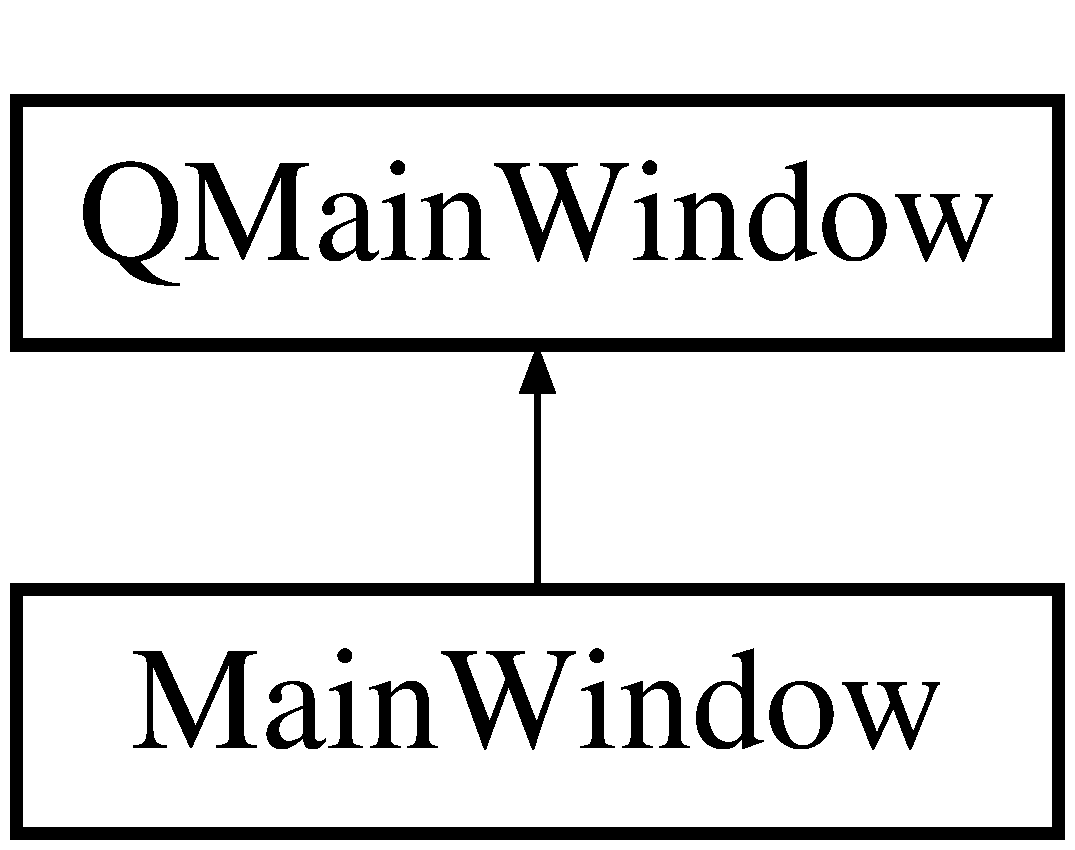
\includegraphics[height=2.000000cm]{classMainWindow}
\end{center}
\end{figure}
\subsection*{Public Slots}
\begin{DoxyCompactItemize}
\item 
void \mbox{\hyperlink{classMainWindow_af61dc400b82ca1d28bab9fb4ee377528}{on\+\_\+ip\+Line\+Edit\+\_\+editing\+Finished}} ()
\begin{DoxyCompactList}\small\item\em Slot recuperant les entrees utilisateur. \end{DoxyCompactList}\item 
void \mbox{\hyperlink{classMainWindow_a4ad002ada4f696aed5badc4728590eea}{on\+\_\+dbname\+Line\+Edit\+\_\+editing\+Finished}} ()
\begin{DoxyCompactList}\small\item\em Slot recuperant les entrees utilisateur. \end{DoxyCompactList}\item 
void \mbox{\hyperlink{classMainWindow_aefd7e7d3ddd36d873d0c972b9d89d0a3}{on\+\_\+dbpwd\+Line\+Edit\+\_\+editing\+Finished}} ()
\begin{DoxyCompactList}\small\item\em Slot recuperant les entrees utilisateur. \end{DoxyCompactList}\item 
void \mbox{\hyperlink{classMainWindow_a33cdc4c422744bb769a725c28b7667d0}{on\+\_\+id\+Line\+Edit\+\_\+editing\+Finished}} ()
\begin{DoxyCompactList}\small\item\em Slot recuperant les entrees utilisateur. \end{DoxyCompactList}\item 
void \mbox{\hyperlink{classMainWindow_a1a1846c640e2e6e208455a85f2c47a04}{on\+\_\+pwd\+Line\+Edit\+\_\+editing\+Finished}} ()
\begin{DoxyCompactList}\small\item\em Slot recuperant les entrees utilisateur. \end{DoxyCompactList}\item 
void \mbox{\hyperlink{classMainWindow_a55cd52e7b00aff669290588f8affea5a}{on\+\_\+connect\+Button\+\_\+clicked}} ()
\begin{DoxyCompactList}\small\item\em Slot effectuant la connexion. \end{DoxyCompactList}\end{DoxyCompactItemize}
\subsection*{Public Member Functions}
\begin{DoxyCompactItemize}
\item 
\mbox{\hyperlink{classMainWindow_a8b244be8b7b7db1b08de2a2acb9409db}{Main\+Window}} (Q\+Widget $\ast$parent=0)
\begin{DoxyCompactList}\small\item\em Constructeur. \end{DoxyCompactList}\item 
\mbox{\hyperlink{classMainWindow_ae98d00a93bc118200eeef9f9bba1dba7}{$\sim$\+Main\+Window}} ()
\begin{DoxyCompactList}\small\item\em Destructeur. \end{DoxyCompactList}\item 
void \mbox{\hyperlink{classMainWindow_ad098a8e0f66eebcdda2a7a1ee7fba382}{read\+Conf\+File}} ()
\begin{DoxyCompactList}\small\item\em Fonction de lecture du fichier de configuration. \end{DoxyCompactList}\end{DoxyCompactItemize}


\subsection{Detailed Description}
Une classe Qt pour gerer la fenetre de connexion. 

La classe met en place la bdd et permet de se connecter pour afficher la fenetre de gestion 

\subsection{Constructor \& Destructor Documentation}
\mbox{\Hypertarget{classMainWindow_a8b244be8b7b7db1b08de2a2acb9409db}\label{classMainWindow_a8b244be8b7b7db1b08de2a2acb9409db}} 
\index{Main\+Window@{Main\+Window}!Main\+Window@{Main\+Window}}
\index{Main\+Window@{Main\+Window}!Main\+Window@{Main\+Window}}
\subsubsection{\texorpdfstring{Main\+Window()}{MainWindow()}}
{\footnotesize\ttfamily Main\+Window\+::\+Main\+Window (\begin{DoxyParamCaption}\item[{Q\+Widget $\ast$}]{parent = {\ttfamily 0} }\end{DoxyParamCaption})\hspace{0.3cm}{\ttfamily [explicit]}}



Constructeur. 

Constructeur de la classe \mbox{\hyperlink{classMainWindow}{Main\+Window}}.


\begin{DoxyParams}{Parameters}
{\em Q\+Widget} & $\ast$parent = 0 \+: Permet de faire passer un widget parent. Par défaut ce parametre vaut 0 \\
\hline
\end{DoxyParams}
\mbox{\Hypertarget{classMainWindow_ae98d00a93bc118200eeef9f9bba1dba7}\label{classMainWindow_ae98d00a93bc118200eeef9f9bba1dba7}} 
\index{Main\+Window@{Main\+Window}!````~Main\+Window@{$\sim$\+Main\+Window}}
\index{````~Main\+Window@{$\sim$\+Main\+Window}!Main\+Window@{Main\+Window}}
\subsubsection{\texorpdfstring{$\sim$\+Main\+Window()}{~MainWindow()}}
{\footnotesize\ttfamily Main\+Window\+::$\sim$\+Main\+Window (\begin{DoxyParamCaption}{ }\end{DoxyParamCaption})}



Destructeur. 

Destructeur de la classe \mbox{\hyperlink{classMainWindow}{Main\+Window}} 

\subsection{Member Function Documentation}
\mbox{\Hypertarget{classMainWindow_a55cd52e7b00aff669290588f8affea5a}\label{classMainWindow_a55cd52e7b00aff669290588f8affea5a}} 
\index{Main\+Window@{Main\+Window}!on\+\_\+connect\+Button\+\_\+clicked@{on\+\_\+connect\+Button\+\_\+clicked}}
\index{on\+\_\+connect\+Button\+\_\+clicked@{on\+\_\+connect\+Button\+\_\+clicked}!Main\+Window@{Main\+Window}}
\subsubsection{\texorpdfstring{on\+\_\+connect\+Button\+\_\+clicked}{on\_connectButton\_clicked}}
{\footnotesize\ttfamily void Main\+Window\+::on\+\_\+connect\+Button\+\_\+clicked (\begin{DoxyParamCaption}{ }\end{DoxyParamCaption})\hspace{0.3cm}{\ttfamily [slot]}}



Slot effectuant la connexion. 

Slot du boutton de connexion. Il permet de gerer les erreurs sur les entrées, creer une classe \mbox{\hyperlink{classDatabase}{Database}} et la fenetre de gestion de la B\+DD. \mbox{\Hypertarget{classMainWindow_a4ad002ada4f696aed5badc4728590eea}\label{classMainWindow_a4ad002ada4f696aed5badc4728590eea}} 
\index{Main\+Window@{Main\+Window}!on\+\_\+dbname\+Line\+Edit\+\_\+editing\+Finished@{on\+\_\+dbname\+Line\+Edit\+\_\+editing\+Finished}}
\index{on\+\_\+dbname\+Line\+Edit\+\_\+editing\+Finished@{on\+\_\+dbname\+Line\+Edit\+\_\+editing\+Finished}!Main\+Window@{Main\+Window}}
\subsubsection{\texorpdfstring{on\+\_\+dbname\+Line\+Edit\+\_\+editing\+Finished}{on\_dbnameLineEdit\_editingFinished}}
{\footnotesize\ttfamily void Main\+Window\+::on\+\_\+dbname\+Line\+Edit\+\_\+editing\+Finished (\begin{DoxyParamCaption}{ }\end{DoxyParamCaption})\hspace{0.3cm}{\ttfamily [slot]}}



Slot recuperant les entrees utilisateur. 

Ce slot stocke dans db\+Name le nom de la bdd entré \mbox{\Hypertarget{classMainWindow_aefd7e7d3ddd36d873d0c972b9d89d0a3}\label{classMainWindow_aefd7e7d3ddd36d873d0c972b9d89d0a3}} 
\index{Main\+Window@{Main\+Window}!on\+\_\+dbpwd\+Line\+Edit\+\_\+editing\+Finished@{on\+\_\+dbpwd\+Line\+Edit\+\_\+editing\+Finished}}
\index{on\+\_\+dbpwd\+Line\+Edit\+\_\+editing\+Finished@{on\+\_\+dbpwd\+Line\+Edit\+\_\+editing\+Finished}!Main\+Window@{Main\+Window}}
\subsubsection{\texorpdfstring{on\+\_\+dbpwd\+Line\+Edit\+\_\+editing\+Finished}{on\_dbpwdLineEdit\_editingFinished}}
{\footnotesize\ttfamily void Main\+Window\+::on\+\_\+dbpwd\+Line\+Edit\+\_\+editing\+Finished (\begin{DoxyParamCaption}{ }\end{DoxyParamCaption})\hspace{0.3cm}{\ttfamily [slot]}}



Slot recuperant les entrees utilisateur. 

Ce slot stocke dans db\+Pwd le mot de passe de la bdd entré \mbox{\Hypertarget{classMainWindow_a33cdc4c422744bb769a725c28b7667d0}\label{classMainWindow_a33cdc4c422744bb769a725c28b7667d0}} 
\index{Main\+Window@{Main\+Window}!on\+\_\+id\+Line\+Edit\+\_\+editing\+Finished@{on\+\_\+id\+Line\+Edit\+\_\+editing\+Finished}}
\index{on\+\_\+id\+Line\+Edit\+\_\+editing\+Finished@{on\+\_\+id\+Line\+Edit\+\_\+editing\+Finished}!Main\+Window@{Main\+Window}}
\subsubsection{\texorpdfstring{on\+\_\+id\+Line\+Edit\+\_\+editing\+Finished}{on\_idLineEdit\_editingFinished}}
{\footnotesize\ttfamily void Main\+Window\+::on\+\_\+id\+Line\+Edit\+\_\+editing\+Finished (\begin{DoxyParamCaption}{ }\end{DoxyParamCaption})\hspace{0.3cm}{\ttfamily [slot]}}



Slot recuperant les entrees utilisateur. 

Ce slot stocke dans user le nom d\textquotesingle{}utilisateur entré \mbox{\Hypertarget{classMainWindow_af61dc400b82ca1d28bab9fb4ee377528}\label{classMainWindow_af61dc400b82ca1d28bab9fb4ee377528}} 
\index{Main\+Window@{Main\+Window}!on\+\_\+ip\+Line\+Edit\+\_\+editing\+Finished@{on\+\_\+ip\+Line\+Edit\+\_\+editing\+Finished}}
\index{on\+\_\+ip\+Line\+Edit\+\_\+editing\+Finished@{on\+\_\+ip\+Line\+Edit\+\_\+editing\+Finished}!Main\+Window@{Main\+Window}}
\subsubsection{\texorpdfstring{on\+\_\+ip\+Line\+Edit\+\_\+editing\+Finished}{on\_ipLineEdit\_editingFinished}}
{\footnotesize\ttfamily void Main\+Window\+::on\+\_\+ip\+Line\+Edit\+\_\+editing\+Finished (\begin{DoxyParamCaption}{ }\end{DoxyParamCaption})\hspace{0.3cm}{\ttfamily [slot]}}



Slot recuperant les entrees utilisateur. 

Ce slot stocke dans ip\+Address l\textquotesingle{}ip entrée \mbox{\Hypertarget{classMainWindow_a1a1846c640e2e6e208455a85f2c47a04}\label{classMainWindow_a1a1846c640e2e6e208455a85f2c47a04}} 
\index{Main\+Window@{Main\+Window}!on\+\_\+pwd\+Line\+Edit\+\_\+editing\+Finished@{on\+\_\+pwd\+Line\+Edit\+\_\+editing\+Finished}}
\index{on\+\_\+pwd\+Line\+Edit\+\_\+editing\+Finished@{on\+\_\+pwd\+Line\+Edit\+\_\+editing\+Finished}!Main\+Window@{Main\+Window}}
\subsubsection{\texorpdfstring{on\+\_\+pwd\+Line\+Edit\+\_\+editing\+Finished}{on\_pwdLineEdit\_editingFinished}}
{\footnotesize\ttfamily void Main\+Window\+::on\+\_\+pwd\+Line\+Edit\+\_\+editing\+Finished (\begin{DoxyParamCaption}{ }\end{DoxyParamCaption})\hspace{0.3cm}{\ttfamily [slot]}}



Slot recuperant les entrees utilisateur. 

Ce slot stocke dans pwd le mot de passe entré \mbox{\Hypertarget{classMainWindow_ad098a8e0f66eebcdda2a7a1ee7fba382}\label{classMainWindow_ad098a8e0f66eebcdda2a7a1ee7fba382}} 
\index{Main\+Window@{Main\+Window}!read\+Conf\+File@{read\+Conf\+File}}
\index{read\+Conf\+File@{read\+Conf\+File}!Main\+Window@{Main\+Window}}
\subsubsection{\texorpdfstring{read\+Conf\+File()}{readConfFile()}}
{\footnotesize\ttfamily void Main\+Window\+::read\+Conf\+File (\begin{DoxyParamCaption}{ }\end{DoxyParamCaption})}



Fonction de lecture du fichier de configuration. 

Cette fonction lit le fichier de configuration et en extrait les données pour remplir les champs d\textquotesingle{}entrée d\textquotesingle{}ip et du nom de la bdd 

The documentation for this class was generated from the following files\+:\begin{DoxyCompactItemize}
\item 
Headers/\mbox{\hyperlink{mainwindow_8hpp}{mainwindow.\+hpp}}\item 
Sources/\mbox{\hyperlink{mainwindow_8cpp}{mainwindow.\+cpp}}\end{DoxyCompactItemize}

\hypertarget{classManageWindow}{}\section{Manage\+Window Class Reference}
\label{classManageWindow}\index{Manage\+Window@{Manage\+Window}}


Une classe Qt pour gerer la fenetre de gestion de la B\+DD.  




{\ttfamily \#include $<$managewindow.\+hpp$>$}

Inheritance diagram for Manage\+Window\+:\begin{figure}[H]
\begin{center}
\leavevmode
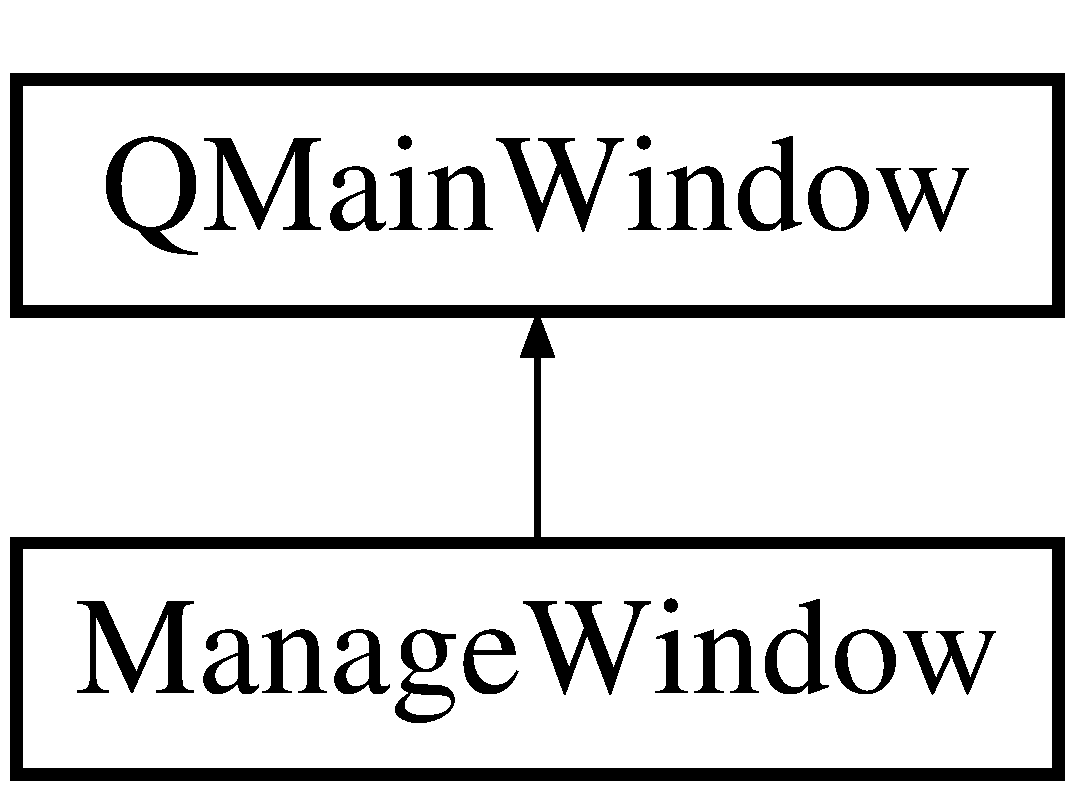
\includegraphics[height=2.000000cm]{classManageWindow}
\end{center}
\end{figure}
\subsection*{Public Slots}
\begin{DoxyCompactItemize}
\item 
void \mbox{\hyperlink{classManageWindow_aa8300cda04fa827c9335fa58a4286528}{on\+\_\+logout\+Button\+\_\+clicked}} ()
\begin{DoxyCompactList}\small\item\em Slot du bouton de deconnexion. \end{DoxyCompactList}\item 
void \mbox{\hyperlink{classManageWindow_a125df0273d83768ef398e20b95dc1f27}{on\+\_\+theme\+Picker\+\_\+activated}} (const Q\+String \&statement)
\begin{DoxyCompactList}\small\item\em Slots de Q\+Combo\+Box. \end{DoxyCompactList}\item 
void \mbox{\hyperlink{classManageWindow_a57fb9a37381bb5498c55b719a258d869}{on\+\_\+theme\+Picker2\+\_\+activated}} (const Q\+String \&statement)
\begin{DoxyCompactList}\small\item\em Slots de Q\+Combo\+Box. \end{DoxyCompactList}\item 
void \mbox{\hyperlink{classManageWindow_aebb1e761d8f734bd825bf07926b82bd1}{on\+\_\+question\+Picker\+\_\+activated}} (const Q\+String \&statement)
\begin{DoxyCompactList}\small\item\em Slots de Q\+Combo\+Box. \end{DoxyCompactList}\item 
void \mbox{\hyperlink{classManageWindow_ac4bafce26b6113a4490f5609e8cdd17b}{on\+\_\+prop\+Picker\+\_\+activated}} (const Q\+String \&statement)
\begin{DoxyCompactList}\small\item\em Slots de Q\+Combo\+Box. \end{DoxyCompactList}\item 
void \mbox{\hyperlink{classManageWindow_a5aeb8691ae16f640a8d22809459a7a9d}{on\+\_\+user\+Picker\+\_\+activated}} (const Q\+String \&statement)
\begin{DoxyCompactList}\small\item\em Slots de Q\+Combo\+Box. \end{DoxyCompactList}\item 
void \mbox{\hyperlink{classManageWindow_a04e344f40ac0714f5ae807499b58ad2d}{on\+\_\+new\+Theme\+Line\+Edit\+\_\+editing\+Finished}} ()
\begin{DoxyCompactList}\small\item\em Slots des Q\+Line\+Edit d\textquotesingle{}ajout. \end{DoxyCompactList}\item 
void \mbox{\hyperlink{classManageWindow_a7aa50da39db54a80f5cc1462bf830657}{on\+\_\+add\+Question\+Line\+Edit\+\_\+editing\+Finished}} ()
\begin{DoxyCompactList}\small\item\em Slot de Q\+Line\+Edit d\textquotesingle{}ajout. \end{DoxyCompactList}\item 
void \mbox{\hyperlink{classManageWindow_abcb9c2271d2726392ba811775ebcc685}{on\+\_\+add\+Prop\+Line\+Edit\+\_\+editing\+Finished}} ()
\begin{DoxyCompactList}\small\item\em Slot de Q\+Line\+Edit d\textquotesingle{}ajout. \end{DoxyCompactList}\item 
void \mbox{\hyperlink{classManageWindow_ac66c5947e1a7e97e82b860471f185fa1}{on\+\_\+add\+Prop\+Line\+Edit2\+\_\+editing\+Finished}} ()
\begin{DoxyCompactList}\small\item\em Slot de Q\+Line\+Edit d\textquotesingle{}ajout. \end{DoxyCompactList}\item 
void \mbox{\hyperlink{classManageWindow_a9d53e0e1ca6c02d197d3b44926dbd5b7}{on\+\_\+new\+Username\+Line\+Edit\+\_\+editing\+Finished}} ()
\begin{DoxyCompactList}\small\item\em Slot de Q\+Line\+Edit d\textquotesingle{}ajout. \end{DoxyCompactList}\item 
void \mbox{\hyperlink{classManageWindow_a859f6ebcd55bb08d3013fd25fa902304}{on\+\_\+new\+Pwd\+Line\+Edit\+\_\+editing\+Finished}} ()
\begin{DoxyCompactList}\small\item\em Slot de Q\+Line\+Edit d\textquotesingle{}ajout. \end{DoxyCompactList}\item 
void \mbox{\hyperlink{classManageWindow_a642bd872d6a3e0ff95cc41cd57d4baa2}{on\+\_\+theme\+Line\+Edit\+\_\+editing\+Finished}} ()
\begin{DoxyCompactList}\small\item\em Slot de Q\+Line\+Edit d\textquotesingle{}edition. \end{DoxyCompactList}\item 
void \mbox{\hyperlink{classManageWindow_a9073026764e994ee447cc68fc4c97521}{on\+\_\+edit\+Question\+Line\+Edit\+\_\+editing\+Finished}} ()
\begin{DoxyCompactList}\small\item\em Slot de Q\+Line\+Edit d\textquotesingle{}edition. \end{DoxyCompactList}\item 
void \mbox{\hyperlink{classManageWindow_aa6223c4f4deb479dd97dc386e6425a6a}{on\+\_\+edit\+Prop\+Line\+Edit\+\_\+editing\+Finished}} ()
\begin{DoxyCompactList}\small\item\em Slot de Q\+Line\+Edit d\textquotesingle{}edition. \end{DoxyCompactList}\item 
void \mbox{\hyperlink{classManageWindow_ac8f74ba7697067a0aaadabd04675093e}{on\+\_\+username\+Line\+Edit\+\_\+editing\+Finished}} ()
\begin{DoxyCompactList}\small\item\em Slot de Q\+Line\+Edit d\textquotesingle{}edition. \end{DoxyCompactList}\item 
void \mbox{\hyperlink{classManageWindow_ab8ca1c057dcd2d277a3540a66cd9145c}{on\+\_\+pwd\+Line\+Edit\+\_\+editing\+Finished}} ()
\begin{DoxyCompactList}\small\item\em Slot de Q\+Line\+Edit d\textquotesingle{}edition. \end{DoxyCompactList}\item 
void \mbox{\hyperlink{classManageWindow_ab2651b6595618b6c1c1789328d47cd35}{on\+\_\+test\+Admin\+Checkbox\+\_\+state\+Changed}} (int state)
\begin{DoxyCompactList}\small\item\em Slot de Q\+Check\+Box. \end{DoxyCompactList}\item 
void \mbox{\hyperlink{classManageWindow_ab7d59fdc4c2c9a5e87a35bbd2dc347eb}{on\+\_\+make\+Admin\+Check\+Box\+\_\+state\+Changed}} (int state)
\begin{DoxyCompactList}\small\item\em Slot de Q\+Check\+Box. \end{DoxyCompactList}\item 
void \mbox{\hyperlink{classManageWindow_a77d7f3c9d65fa3e1842778aa554c3d19}{on\+\_\+add\+Theme\+Button\+\_\+clicked}} ()
\begin{DoxyCompactList}\small\item\em Slot des bouton d\textquotesingle{}ajout. \end{DoxyCompactList}\item 
void \mbox{\hyperlink{classManageWindow_a5f84c69a12caf2a8b934b5ed59a30f88}{on\+\_\+add\+Question\+Button\+\_\+clicked}} ()
\begin{DoxyCompactList}\small\item\em Slot des bouton d\textquotesingle{}ajout. \end{DoxyCompactList}\item 
void \mbox{\hyperlink{classManageWindow_a28475c18e491f3e388747685731e5111}{on\+\_\+add\+Prop\+Button\+\_\+clicked}} ()
\begin{DoxyCompactList}\small\item\em Slot des bouton d\textquotesingle{}ajout. \end{DoxyCompactList}\item 
void \mbox{\hyperlink{classManageWindow_a7b65c7bb9f7d022d57575db22a8e8e00}{on\+\_\+add\+Prop\+Button2\+\_\+clicked}} ()
\begin{DoxyCompactList}\small\item\em Slot des bouton d\textquotesingle{}ajout. \end{DoxyCompactList}\item 
void \mbox{\hyperlink{classManageWindow_a741f69a15264a0b10767cc89522ecaf9}{on\+\_\+add\+User\+Button\+\_\+clicked}} ()
\begin{DoxyCompactList}\small\item\em Slot des bouton d\textquotesingle{}ajout. \end{DoxyCompactList}\item 
void \mbox{\hyperlink{classManageWindow_aed7adfd94929cb522de43f1aa3314483}{on\+\_\+theme\+Edit\+Button\+\_\+clicked}} ()
\begin{DoxyCompactList}\small\item\em Slot des bouton d\textquotesingle{}edition. \end{DoxyCompactList}\item 
void \mbox{\hyperlink{classManageWindow_a302b93485498f6bfbe5c362298222620}{on\+\_\+edit\+Question\+Button\+\_\+clicked}} ()
\begin{DoxyCompactList}\small\item\em Slot des bouton d\textquotesingle{}edition. \end{DoxyCompactList}\item 
void \mbox{\hyperlink{classManageWindow_a5ca2c828847bf13c40699128cc061171}{on\+\_\+edit\+Prop\+Button\+\_\+clicked}} ()
\begin{DoxyCompactList}\small\item\em Slot des bouton d\textquotesingle{}edition. \end{DoxyCompactList}\item 
void \mbox{\hyperlink{classManageWindow_a4904b87aefc385fe5343f93fde153a2a}{on\+\_\+edit\+User\+Push\+Button\+\_\+clicked}} ()
\begin{DoxyCompactList}\small\item\em Slot des bouton d\textquotesingle{}edition. \end{DoxyCompactList}\item 
void \mbox{\hyperlink{classManageWindow_a89f9fbc2426fb7c3afb890ef446c2161}{on\+\_\+delete\+Theme\+Button\+\_\+clicked}} ()
\begin{DoxyCompactList}\small\item\em Slot des bouton de suppression. \end{DoxyCompactList}\item 
void \mbox{\hyperlink{classManageWindow_a9eba7473d0b4bacf9767629537672778}{on\+\_\+delete\+Question\+Button\+\_\+clicked}} ()
\begin{DoxyCompactList}\small\item\em Slot des bouton de suppression. \end{DoxyCompactList}\item 
void \mbox{\hyperlink{classManageWindow_ac191196301dfcbb30d995790a7e5e496}{on\+\_\+delete\+Prop\+Button\+\_\+clicked}} ()
\begin{DoxyCompactList}\small\item\em Slot des bouton de suppression. \end{DoxyCompactList}\item 
void \mbox{\hyperlink{classManageWindow_a23bbad3a8c73d95e2f8f27df6458d2ea}{on\+\_\+delete\+User\+Button\+\_\+clicked}} ()
\begin{DoxyCompactList}\small\item\em Slot des bouton de suppression. \end{DoxyCompactList}\end{DoxyCompactItemize}
\subsection*{Public Member Functions}
\begin{DoxyCompactItemize}
\item 
\mbox{\hyperlink{classManageWindow_ab5bd55471f7e1a749810dd28fcc7b9c0}{Manage\+Window}} (\mbox{\hyperlink{classDatabase}{Database}} $\ast$dtb, Q\+Widget $\ast$parent=0)
\begin{DoxyCompactList}\small\item\em Constructeur. \end{DoxyCompactList}\item 
\mbox{\hyperlink{classManageWindow_a7ce02d4018de7f914756c13aa5b965fd}{$\sim$\+Manage\+Window}} ()
\begin{DoxyCompactList}\small\item\em Destructeur. \end{DoxyCompactList}\item 
bool \mbox{\hyperlink{classManageWindow_aac50125bb2e62a8e9905c4c5a09c6184}{check\+Syntax}} (string question)
\begin{DoxyCompactList}\small\item\em Verification de syntaxe. \end{DoxyCompactList}\item 
void \mbox{\hyperlink{classManageWindow_a746f794bbc9b2aa007fc4ccd2a8504d8}{fill\+Pickers}} ()
\begin{DoxyCompactList}\small\item\em Fonction de remplissage de Q\+Combo\+Box. \end{DoxyCompactList}\item 
void \mbox{\hyperlink{classManageWindow_a1ce0be0aaeb2a8809004aa6a0316c6b9}{fill\+Theme\+Picker2}} ()
\begin{DoxyCompactList}\small\item\em Fonction de remplissage de Q\+Combo\+Box. \end{DoxyCompactList}\item 
void \mbox{\hyperlink{classManageWindow_a1276d421282259be54035b2137a71ccf}{fill\+Answer\+Picker}} (string question)
\begin{DoxyCompactList}\small\item\em Fonction de remplissage de Q\+Combo\+Box. \end{DoxyCompactList}\item 
void \mbox{\hyperlink{classManageWindow_a40b1c990354a0df80a73889eb78dc02b}{fill\+Answer\+Picker23}} (string question)
\begin{DoxyCompactList}\small\item\em Fonction de remplissage de Q\+Combo\+Box. \end{DoxyCompactList}\item 
void \mbox{\hyperlink{classManageWindow_a08c2bb9ab812720b59794f4eaeb2156b}{fill\+Prop\+Picker}} (string question)
\begin{DoxyCompactList}\small\item\em Fonction de remplissage de Q\+Combo\+Box. \end{DoxyCompactList}\item 
void \mbox{\hyperlink{classManageWindow_a6131d13ca6962964ce8c6a37edbc4006}{fill\+User\+Picker}} ()
\begin{DoxyCompactList}\small\item\em Fonction de remplissage de Q\+Combo\+Box. \end{DoxyCompactList}\end{DoxyCompactItemize}


\subsection{Detailed Description}
Une classe Qt pour gerer la fenetre de gestion de la B\+DD. 

La classe met en place la bdd et permet de se connecter pour afficher la fenetre de gestion 

\subsection{Constructor \& Destructor Documentation}
\mbox{\Hypertarget{classManageWindow_ab5bd55471f7e1a749810dd28fcc7b9c0}\label{classManageWindow_ab5bd55471f7e1a749810dd28fcc7b9c0}} 
\index{Manage\+Window@{Manage\+Window}!Manage\+Window@{Manage\+Window}}
\index{Manage\+Window@{Manage\+Window}!Manage\+Window@{Manage\+Window}}
\subsubsection{\texorpdfstring{Manage\+Window()}{ManageWindow()}}
{\footnotesize\ttfamily Manage\+Window\+::\+Manage\+Window (\begin{DoxyParamCaption}\item[{\mbox{\hyperlink{classDatabase}{Database}} $\ast$}]{dtb,  }\item[{Q\+Widget $\ast$}]{parent = {\ttfamily 0} }\end{DoxyParamCaption})\hspace{0.3cm}{\ttfamily [explicit]}}



Constructeur. 

Constructeur de la classe \mbox{\hyperlink{classManageWindow}{Manage\+Window}}.


\begin{DoxyParams}{Parameters}
{\em \mbox{\hyperlink{classDatabase}{Database}}} & $\ast$dtb \+: Pointeur sur la base de donnée crée dans \mbox{\hyperlink{mainwindow_8cpp}{mainwindow.\+cpp}} \\
\hline
{\em Q\+Widget} & $\ast$parent = 0 \+: Pointeur sur la fenetre de connexion. Par défaut ce parametre vaut 0 \\
\hline
\end{DoxyParams}
\mbox{\Hypertarget{classManageWindow_a7ce02d4018de7f914756c13aa5b965fd}\label{classManageWindow_a7ce02d4018de7f914756c13aa5b965fd}} 
\index{Manage\+Window@{Manage\+Window}!````~Manage\+Window@{$\sim$\+Manage\+Window}}
\index{````~Manage\+Window@{$\sim$\+Manage\+Window}!Manage\+Window@{Manage\+Window}}
\subsubsection{\texorpdfstring{$\sim$\+Manage\+Window()}{~ManageWindow()}}
{\footnotesize\ttfamily Manage\+Window\+::$\sim$\+Manage\+Window (\begin{DoxyParamCaption}{ }\end{DoxyParamCaption})}



Destructeur. 

Destructeur de la classe \mbox{\hyperlink{classManageWindow}{Manage\+Window}} 

\subsection{Member Function Documentation}
\mbox{\Hypertarget{classManageWindow_aac50125bb2e62a8e9905c4c5a09c6184}\label{classManageWindow_aac50125bb2e62a8e9905c4c5a09c6184}} 
\index{Manage\+Window@{Manage\+Window}!check\+Syntax@{check\+Syntax}}
\index{check\+Syntax@{check\+Syntax}!Manage\+Window@{Manage\+Window}}
\subsubsection{\texorpdfstring{check\+Syntax()}{checkSyntax()}}
{\footnotesize\ttfamily bool Manage\+Window\+::check\+Syntax (\begin{DoxyParamCaption}\item[{string}]{question }\end{DoxyParamCaption})}



Verification de syntaxe. 

Cette fonction permet de verifier si une question a bien 2 virgules 
\begin{DoxyParams}{Parameters}
{\em std\+::string} & question \+: La chaine a verifier \\
\hline
\end{DoxyParams}
\begin{DoxyReturn}{Returns}
int 1 \+: La chaine contient 2 virgules 

int 0 \+: La chaine ne contient pas 2 virgules 
\end{DoxyReturn}
\mbox{\Hypertarget{classManageWindow_a1276d421282259be54035b2137a71ccf}\label{classManageWindow_a1276d421282259be54035b2137a71ccf}} 
\index{Manage\+Window@{Manage\+Window}!fill\+Answer\+Picker@{fill\+Answer\+Picker}}
\index{fill\+Answer\+Picker@{fill\+Answer\+Picker}!Manage\+Window@{Manage\+Window}}
\subsubsection{\texorpdfstring{fill\+Answer\+Picker()}{fillAnswerPicker()}}
{\footnotesize\ttfamily void Manage\+Window\+::fill\+Answer\+Picker (\begin{DoxyParamCaption}\item[{string}]{question }\end{DoxyParamCaption})}



Fonction de remplissage de Q\+Combo\+Box. 

Cette fonction permet de remplir le selecteur de bonne reponse dans l\textquotesingle{}ajout de question 
\begin{DoxyParams}{Parameters}
{\em std\+::string} & question \+: La question a decouper pour remplir le selecteur \\
\hline
\end{DoxyParams}
\mbox{\Hypertarget{classManageWindow_a40b1c990354a0df80a73889eb78dc02b}\label{classManageWindow_a40b1c990354a0df80a73889eb78dc02b}} 
\index{Manage\+Window@{Manage\+Window}!fill\+Answer\+Picker23@{fill\+Answer\+Picker23}}
\index{fill\+Answer\+Picker23@{fill\+Answer\+Picker23}!Manage\+Window@{Manage\+Window}}
\subsubsection{\texorpdfstring{fill\+Answer\+Picker23()}{fillAnswerPicker23()}}
{\footnotesize\ttfamily void Manage\+Window\+::fill\+Answer\+Picker23 (\begin{DoxyParamCaption}\item[{string}]{question }\end{DoxyParamCaption})}



Fonction de remplissage de Q\+Combo\+Box. 

Cette fonction permet de remplir le selecteur de bonne reponse dans l\textquotesingle{}edition de question 
\begin{DoxyParams}{Parameters}
{\em std\+::string} & question \+: La question a decouper pour remplir le selecteur \\
\hline
\end{DoxyParams}
\mbox{\Hypertarget{classManageWindow_a746f794bbc9b2aa007fc4ccd2a8504d8}\label{classManageWindow_a746f794bbc9b2aa007fc4ccd2a8504d8}} 
\index{Manage\+Window@{Manage\+Window}!fill\+Pickers@{fill\+Pickers}}
\index{fill\+Pickers@{fill\+Pickers}!Manage\+Window@{Manage\+Window}}
\subsubsection{\texorpdfstring{fill\+Pickers()}{fillPickers()}}
{\footnotesize\ttfamily void Manage\+Window\+::fill\+Pickers (\begin{DoxyParamCaption}{ }\end{DoxyParamCaption})}



Fonction de remplissage de Q\+Combo\+Box. 

Cette fonction permet de remplir le selecteur de themes et de questions \mbox{\Hypertarget{classManageWindow_a08c2bb9ab812720b59794f4eaeb2156b}\label{classManageWindow_a08c2bb9ab812720b59794f4eaeb2156b}} 
\index{Manage\+Window@{Manage\+Window}!fill\+Prop\+Picker@{fill\+Prop\+Picker}}
\index{fill\+Prop\+Picker@{fill\+Prop\+Picker}!Manage\+Window@{Manage\+Window}}
\subsubsection{\texorpdfstring{fill\+Prop\+Picker()}{fillPropPicker()}}
{\footnotesize\ttfamily void Manage\+Window\+::fill\+Prop\+Picker (\begin{DoxyParamCaption}\item[{string}]{question }\end{DoxyParamCaption})}



Fonction de remplissage de Q\+Combo\+Box. 

Cette fonction permet de remplir le selecteur de propositions dans l\textquotesingle{}édition de questions 
\begin{DoxyParams}{Parameters}
{\em std\+::string} & question \+: La question selectionnée \\
\hline
\end{DoxyParams}
\mbox{\Hypertarget{classManageWindow_a1ce0be0aaeb2a8809004aa6a0316c6b9}\label{classManageWindow_a1ce0be0aaeb2a8809004aa6a0316c6b9}} 
\index{Manage\+Window@{Manage\+Window}!fill\+Theme\+Picker2@{fill\+Theme\+Picker2}}
\index{fill\+Theme\+Picker2@{fill\+Theme\+Picker2}!Manage\+Window@{Manage\+Window}}
\subsubsection{\texorpdfstring{fill\+Theme\+Picker2()}{fillThemePicker2()}}
{\footnotesize\ttfamily void Manage\+Window\+::fill\+Theme\+Picker2 (\begin{DoxyParamCaption}{ }\end{DoxyParamCaption})}



Fonction de remplissage de Q\+Combo\+Box. 

Cette fonction permet de remplir le selecteur de theme dans l\textquotesingle{}ajout de questions \mbox{\Hypertarget{classManageWindow_a6131d13ca6962964ce8c6a37edbc4006}\label{classManageWindow_a6131d13ca6962964ce8c6a37edbc4006}} 
\index{Manage\+Window@{Manage\+Window}!fill\+User\+Picker@{fill\+User\+Picker}}
\index{fill\+User\+Picker@{fill\+User\+Picker}!Manage\+Window@{Manage\+Window}}
\subsubsection{\texorpdfstring{fill\+User\+Picker()}{fillUserPicker()}}
{\footnotesize\ttfamily void Manage\+Window\+::fill\+User\+Picker (\begin{DoxyParamCaption}{ }\end{DoxyParamCaption})}



Fonction de remplissage de Q\+Combo\+Box. 

Cette fonction permet de remplir le selecteur d\textquotesingle{}utilisateur \mbox{\Hypertarget{classManageWindow_a7b65c7bb9f7d022d57575db22a8e8e00}\label{classManageWindow_a7b65c7bb9f7d022d57575db22a8e8e00}} 
\index{Manage\+Window@{Manage\+Window}!on\+\_\+add\+Prop\+Button2\+\_\+clicked@{on\+\_\+add\+Prop\+Button2\+\_\+clicked}}
\index{on\+\_\+add\+Prop\+Button2\+\_\+clicked@{on\+\_\+add\+Prop\+Button2\+\_\+clicked}!Manage\+Window@{Manage\+Window}}
\subsubsection{\texorpdfstring{on\+\_\+add\+Prop\+Button2\+\_\+clicked}{on\_addPropButton2\_clicked}}
{\footnotesize\ttfamily void Manage\+Window\+::on\+\_\+add\+Prop\+Button2\+\_\+clicked (\begin{DoxyParamCaption}{ }\end{DoxyParamCaption})\hspace{0.3cm}{\ttfamily [slot]}}



Slot des bouton d\textquotesingle{}ajout. 

Ce slot permet d\textquotesingle{}ajouter une proposition lorsqu\textquotesingle{}il est cliqué après des vérifications \mbox{\Hypertarget{classManageWindow_a28475c18e491f3e388747685731e5111}\label{classManageWindow_a28475c18e491f3e388747685731e5111}} 
\index{Manage\+Window@{Manage\+Window}!on\+\_\+add\+Prop\+Button\+\_\+clicked@{on\+\_\+add\+Prop\+Button\+\_\+clicked}}
\index{on\+\_\+add\+Prop\+Button\+\_\+clicked@{on\+\_\+add\+Prop\+Button\+\_\+clicked}!Manage\+Window@{Manage\+Window}}
\subsubsection{\texorpdfstring{on\+\_\+add\+Prop\+Button\+\_\+clicked}{on\_addPropButton\_clicked}}
{\footnotesize\ttfamily void Manage\+Window\+::on\+\_\+add\+Prop\+Button\+\_\+clicked (\begin{DoxyParamCaption}{ }\end{DoxyParamCaption})\hspace{0.3cm}{\ttfamily [slot]}}



Slot des bouton d\textquotesingle{}ajout. 

Ce slot permet d\textquotesingle{}ajouter une proposition lorsqu\textquotesingle{}il est cliqué après des vérifications \mbox{\Hypertarget{classManageWindow_ac66c5947e1a7e97e82b860471f185fa1}\label{classManageWindow_ac66c5947e1a7e97e82b860471f185fa1}} 
\index{Manage\+Window@{Manage\+Window}!on\+\_\+add\+Prop\+Line\+Edit2\+\_\+editing\+Finished@{on\+\_\+add\+Prop\+Line\+Edit2\+\_\+editing\+Finished}}
\index{on\+\_\+add\+Prop\+Line\+Edit2\+\_\+editing\+Finished@{on\+\_\+add\+Prop\+Line\+Edit2\+\_\+editing\+Finished}!Manage\+Window@{Manage\+Window}}
\subsubsection{\texorpdfstring{on\+\_\+add\+Prop\+Line\+Edit2\+\_\+editing\+Finished}{on\_addPropLineEdit2\_editingFinished}}
{\footnotesize\ttfamily void Manage\+Window\+::on\+\_\+add\+Prop\+Line\+Edit2\+\_\+editing\+Finished (\begin{DoxyParamCaption}{ }\end{DoxyParamCaption})\hspace{0.3cm}{\ttfamily [slot]}}



Slot de Q\+Line\+Edit d\textquotesingle{}ajout. 

Ce slot permet d\textquotesingle{}entrer le nom de la proposition a ajouter \mbox{\Hypertarget{classManageWindow_abcb9c2271d2726392ba811775ebcc685}\label{classManageWindow_abcb9c2271d2726392ba811775ebcc685}} 
\index{Manage\+Window@{Manage\+Window}!on\+\_\+add\+Prop\+Line\+Edit\+\_\+editing\+Finished@{on\+\_\+add\+Prop\+Line\+Edit\+\_\+editing\+Finished}}
\index{on\+\_\+add\+Prop\+Line\+Edit\+\_\+editing\+Finished@{on\+\_\+add\+Prop\+Line\+Edit\+\_\+editing\+Finished}!Manage\+Window@{Manage\+Window}}
\subsubsection{\texorpdfstring{on\+\_\+add\+Prop\+Line\+Edit\+\_\+editing\+Finished}{on\_addPropLineEdit\_editingFinished}}
{\footnotesize\ttfamily void Manage\+Window\+::on\+\_\+add\+Prop\+Line\+Edit\+\_\+editing\+Finished (\begin{DoxyParamCaption}{ }\end{DoxyParamCaption})\hspace{0.3cm}{\ttfamily [slot]}}



Slot de Q\+Line\+Edit d\textquotesingle{}ajout. 

Ce slot permet d\textquotesingle{}entrer le nom de la proposition a ajouter \mbox{\Hypertarget{classManageWindow_a5f84c69a12caf2a8b934b5ed59a30f88}\label{classManageWindow_a5f84c69a12caf2a8b934b5ed59a30f88}} 
\index{Manage\+Window@{Manage\+Window}!on\+\_\+add\+Question\+Button\+\_\+clicked@{on\+\_\+add\+Question\+Button\+\_\+clicked}}
\index{on\+\_\+add\+Question\+Button\+\_\+clicked@{on\+\_\+add\+Question\+Button\+\_\+clicked}!Manage\+Window@{Manage\+Window}}
\subsubsection{\texorpdfstring{on\+\_\+add\+Question\+Button\+\_\+clicked}{on\_addQuestionButton\_clicked}}
{\footnotesize\ttfamily void Manage\+Window\+::on\+\_\+add\+Question\+Button\+\_\+clicked (\begin{DoxyParamCaption}{ }\end{DoxyParamCaption})\hspace{0.3cm}{\ttfamily [slot]}}



Slot des bouton d\textquotesingle{}ajout. 

Ce slot permet d\textquotesingle{}ajouter une question lorsqu\textquotesingle{}il est cliqué après des vérifications \mbox{\Hypertarget{classManageWindow_a7aa50da39db54a80f5cc1462bf830657}\label{classManageWindow_a7aa50da39db54a80f5cc1462bf830657}} 
\index{Manage\+Window@{Manage\+Window}!on\+\_\+add\+Question\+Line\+Edit\+\_\+editing\+Finished@{on\+\_\+add\+Question\+Line\+Edit\+\_\+editing\+Finished}}
\index{on\+\_\+add\+Question\+Line\+Edit\+\_\+editing\+Finished@{on\+\_\+add\+Question\+Line\+Edit\+\_\+editing\+Finished}!Manage\+Window@{Manage\+Window}}
\subsubsection{\texorpdfstring{on\+\_\+add\+Question\+Line\+Edit\+\_\+editing\+Finished}{on\_addQuestionLineEdit\_editingFinished}}
{\footnotesize\ttfamily void Manage\+Window\+::on\+\_\+add\+Question\+Line\+Edit\+\_\+editing\+Finished (\begin{DoxyParamCaption}{ }\end{DoxyParamCaption})\hspace{0.3cm}{\ttfamily [slot]}}



Slot de Q\+Line\+Edit d\textquotesingle{}ajout. 

Ce slot permet d\textquotesingle{}entrer le nom de la question a ajouter \mbox{\Hypertarget{classManageWindow_a77d7f3c9d65fa3e1842778aa554c3d19}\label{classManageWindow_a77d7f3c9d65fa3e1842778aa554c3d19}} 
\index{Manage\+Window@{Manage\+Window}!on\+\_\+add\+Theme\+Button\+\_\+clicked@{on\+\_\+add\+Theme\+Button\+\_\+clicked}}
\index{on\+\_\+add\+Theme\+Button\+\_\+clicked@{on\+\_\+add\+Theme\+Button\+\_\+clicked}!Manage\+Window@{Manage\+Window}}
\subsubsection{\texorpdfstring{on\+\_\+add\+Theme\+Button\+\_\+clicked}{on\_addThemeButton\_clicked}}
{\footnotesize\ttfamily void Manage\+Window\+::on\+\_\+add\+Theme\+Button\+\_\+clicked (\begin{DoxyParamCaption}{ }\end{DoxyParamCaption})\hspace{0.3cm}{\ttfamily [slot]}}



Slot des bouton d\textquotesingle{}ajout. 

Ce slot permet d\textquotesingle{}ajouter un theme lorsqu\textquotesingle{}il est cliqué après des vérifications \mbox{\Hypertarget{classManageWindow_a741f69a15264a0b10767cc89522ecaf9}\label{classManageWindow_a741f69a15264a0b10767cc89522ecaf9}} 
\index{Manage\+Window@{Manage\+Window}!on\+\_\+add\+User\+Button\+\_\+clicked@{on\+\_\+add\+User\+Button\+\_\+clicked}}
\index{on\+\_\+add\+User\+Button\+\_\+clicked@{on\+\_\+add\+User\+Button\+\_\+clicked}!Manage\+Window@{Manage\+Window}}
\subsubsection{\texorpdfstring{on\+\_\+add\+User\+Button\+\_\+clicked}{on\_addUserButton\_clicked}}
{\footnotesize\ttfamily void Manage\+Window\+::on\+\_\+add\+User\+Button\+\_\+clicked (\begin{DoxyParamCaption}{ }\end{DoxyParamCaption})\hspace{0.3cm}{\ttfamily [slot]}}



Slot des bouton d\textquotesingle{}ajout. 

Ce slot permet d\textquotesingle{}ajouter un utilisateur lorsqu\textquotesingle{}il est cliqué après des vérifications \mbox{\Hypertarget{classManageWindow_ac191196301dfcbb30d995790a7e5e496}\label{classManageWindow_ac191196301dfcbb30d995790a7e5e496}} 
\index{Manage\+Window@{Manage\+Window}!on\+\_\+delete\+Prop\+Button\+\_\+clicked@{on\+\_\+delete\+Prop\+Button\+\_\+clicked}}
\index{on\+\_\+delete\+Prop\+Button\+\_\+clicked@{on\+\_\+delete\+Prop\+Button\+\_\+clicked}!Manage\+Window@{Manage\+Window}}
\subsubsection{\texorpdfstring{on\+\_\+delete\+Prop\+Button\+\_\+clicked}{on\_deletePropButton\_clicked}}
{\footnotesize\ttfamily void Manage\+Window\+::on\+\_\+delete\+Prop\+Button\+\_\+clicked (\begin{DoxyParamCaption}{ }\end{DoxyParamCaption})\hspace{0.3cm}{\ttfamily [slot]}}



Slot des bouton de suppression. 

Ce slot permet de supprimer une proposition lorsqu\textquotesingle{}il est cliqué après des vérifications \mbox{\Hypertarget{classManageWindow_a9eba7473d0b4bacf9767629537672778}\label{classManageWindow_a9eba7473d0b4bacf9767629537672778}} 
\index{Manage\+Window@{Manage\+Window}!on\+\_\+delete\+Question\+Button\+\_\+clicked@{on\+\_\+delete\+Question\+Button\+\_\+clicked}}
\index{on\+\_\+delete\+Question\+Button\+\_\+clicked@{on\+\_\+delete\+Question\+Button\+\_\+clicked}!Manage\+Window@{Manage\+Window}}
\subsubsection{\texorpdfstring{on\+\_\+delete\+Question\+Button\+\_\+clicked}{on\_deleteQuestionButton\_clicked}}
{\footnotesize\ttfamily void Manage\+Window\+::on\+\_\+delete\+Question\+Button\+\_\+clicked (\begin{DoxyParamCaption}{ }\end{DoxyParamCaption})\hspace{0.3cm}{\ttfamily [slot]}}



Slot des bouton de suppression. 

Ce slot permet de supprimer une question lorsqu\textquotesingle{}il est cliqué après des vérifications \mbox{\Hypertarget{classManageWindow_a89f9fbc2426fb7c3afb890ef446c2161}\label{classManageWindow_a89f9fbc2426fb7c3afb890ef446c2161}} 
\index{Manage\+Window@{Manage\+Window}!on\+\_\+delete\+Theme\+Button\+\_\+clicked@{on\+\_\+delete\+Theme\+Button\+\_\+clicked}}
\index{on\+\_\+delete\+Theme\+Button\+\_\+clicked@{on\+\_\+delete\+Theme\+Button\+\_\+clicked}!Manage\+Window@{Manage\+Window}}
\subsubsection{\texorpdfstring{on\+\_\+delete\+Theme\+Button\+\_\+clicked}{on\_deleteThemeButton\_clicked}}
{\footnotesize\ttfamily void Manage\+Window\+::on\+\_\+delete\+Theme\+Button\+\_\+clicked (\begin{DoxyParamCaption}{ }\end{DoxyParamCaption})\hspace{0.3cm}{\ttfamily [slot]}}



Slot des bouton de suppression. 

Ce slot permet de supprimer un theme lorsqu\textquotesingle{}il est cliqué après des vérifications \mbox{\Hypertarget{classManageWindow_a23bbad3a8c73d95e2f8f27df6458d2ea}\label{classManageWindow_a23bbad3a8c73d95e2f8f27df6458d2ea}} 
\index{Manage\+Window@{Manage\+Window}!on\+\_\+delete\+User\+Button\+\_\+clicked@{on\+\_\+delete\+User\+Button\+\_\+clicked}}
\index{on\+\_\+delete\+User\+Button\+\_\+clicked@{on\+\_\+delete\+User\+Button\+\_\+clicked}!Manage\+Window@{Manage\+Window}}
\subsubsection{\texorpdfstring{on\+\_\+delete\+User\+Button\+\_\+clicked}{on\_deleteUserButton\_clicked}}
{\footnotesize\ttfamily void Manage\+Window\+::on\+\_\+delete\+User\+Button\+\_\+clicked (\begin{DoxyParamCaption}{ }\end{DoxyParamCaption})\hspace{0.3cm}{\ttfamily [slot]}}



Slot des bouton de suppression. 

Ce slot permet de supprimer un utilisateur lorsqu\textquotesingle{}il est cliqué après des vérifications \mbox{\Hypertarget{classManageWindow_a5ca2c828847bf13c40699128cc061171}\label{classManageWindow_a5ca2c828847bf13c40699128cc061171}} 
\index{Manage\+Window@{Manage\+Window}!on\+\_\+edit\+Prop\+Button\+\_\+clicked@{on\+\_\+edit\+Prop\+Button\+\_\+clicked}}
\index{on\+\_\+edit\+Prop\+Button\+\_\+clicked@{on\+\_\+edit\+Prop\+Button\+\_\+clicked}!Manage\+Window@{Manage\+Window}}
\subsubsection{\texorpdfstring{on\+\_\+edit\+Prop\+Button\+\_\+clicked}{on\_editPropButton\_clicked}}
{\footnotesize\ttfamily void Manage\+Window\+::on\+\_\+edit\+Prop\+Button\+\_\+clicked (\begin{DoxyParamCaption}{ }\end{DoxyParamCaption})\hspace{0.3cm}{\ttfamily [slot]}}



Slot des bouton d\textquotesingle{}edition. 

Ce slot permet d\textquotesingle{}editer une proposition lorsqu\textquotesingle{}il est cliqué après des vérifications \mbox{\Hypertarget{classManageWindow_aa6223c4f4deb479dd97dc386e6425a6a}\label{classManageWindow_aa6223c4f4deb479dd97dc386e6425a6a}} 
\index{Manage\+Window@{Manage\+Window}!on\+\_\+edit\+Prop\+Line\+Edit\+\_\+editing\+Finished@{on\+\_\+edit\+Prop\+Line\+Edit\+\_\+editing\+Finished}}
\index{on\+\_\+edit\+Prop\+Line\+Edit\+\_\+editing\+Finished@{on\+\_\+edit\+Prop\+Line\+Edit\+\_\+editing\+Finished}!Manage\+Window@{Manage\+Window}}
\subsubsection{\texorpdfstring{on\+\_\+edit\+Prop\+Line\+Edit\+\_\+editing\+Finished}{on\_editPropLineEdit\_editingFinished}}
{\footnotesize\ttfamily void Manage\+Window\+::on\+\_\+edit\+Prop\+Line\+Edit\+\_\+editing\+Finished (\begin{DoxyParamCaption}{ }\end{DoxyParamCaption})\hspace{0.3cm}{\ttfamily [slot]}}



Slot de Q\+Line\+Edit d\textquotesingle{}edition. 

Ce slot permet d\textquotesingle{}entrer le nouveau nom de la proposition a editer \mbox{\Hypertarget{classManageWindow_a302b93485498f6bfbe5c362298222620}\label{classManageWindow_a302b93485498f6bfbe5c362298222620}} 
\index{Manage\+Window@{Manage\+Window}!on\+\_\+edit\+Question\+Button\+\_\+clicked@{on\+\_\+edit\+Question\+Button\+\_\+clicked}}
\index{on\+\_\+edit\+Question\+Button\+\_\+clicked@{on\+\_\+edit\+Question\+Button\+\_\+clicked}!Manage\+Window@{Manage\+Window}}
\subsubsection{\texorpdfstring{on\+\_\+edit\+Question\+Button\+\_\+clicked}{on\_editQuestionButton\_clicked}}
{\footnotesize\ttfamily void Manage\+Window\+::on\+\_\+edit\+Question\+Button\+\_\+clicked (\begin{DoxyParamCaption}{ }\end{DoxyParamCaption})\hspace{0.3cm}{\ttfamily [slot]}}



Slot des bouton d\textquotesingle{}edition. 

Ce slot permet d\textquotesingle{}editer une question lorsqu\textquotesingle{}il est cliqué après des vérifications \mbox{\Hypertarget{classManageWindow_a9073026764e994ee447cc68fc4c97521}\label{classManageWindow_a9073026764e994ee447cc68fc4c97521}} 
\index{Manage\+Window@{Manage\+Window}!on\+\_\+edit\+Question\+Line\+Edit\+\_\+editing\+Finished@{on\+\_\+edit\+Question\+Line\+Edit\+\_\+editing\+Finished}}
\index{on\+\_\+edit\+Question\+Line\+Edit\+\_\+editing\+Finished@{on\+\_\+edit\+Question\+Line\+Edit\+\_\+editing\+Finished}!Manage\+Window@{Manage\+Window}}
\subsubsection{\texorpdfstring{on\+\_\+edit\+Question\+Line\+Edit\+\_\+editing\+Finished}{on\_editQuestionLineEdit\_editingFinished}}
{\footnotesize\ttfamily void Manage\+Window\+::on\+\_\+edit\+Question\+Line\+Edit\+\_\+editing\+Finished (\begin{DoxyParamCaption}{ }\end{DoxyParamCaption})\hspace{0.3cm}{\ttfamily [slot]}}



Slot de Q\+Line\+Edit d\textquotesingle{}edition. 

Ce slot permet d\textquotesingle{}entrer le nouveau nom de la question a editer \mbox{\Hypertarget{classManageWindow_a4904b87aefc385fe5343f93fde153a2a}\label{classManageWindow_a4904b87aefc385fe5343f93fde153a2a}} 
\index{Manage\+Window@{Manage\+Window}!on\+\_\+edit\+User\+Push\+Button\+\_\+clicked@{on\+\_\+edit\+User\+Push\+Button\+\_\+clicked}}
\index{on\+\_\+edit\+User\+Push\+Button\+\_\+clicked@{on\+\_\+edit\+User\+Push\+Button\+\_\+clicked}!Manage\+Window@{Manage\+Window}}
\subsubsection{\texorpdfstring{on\+\_\+edit\+User\+Push\+Button\+\_\+clicked}{on\_editUserPushButton\_clicked}}
{\footnotesize\ttfamily void Manage\+Window\+::on\+\_\+edit\+User\+Push\+Button\+\_\+clicked (\begin{DoxyParamCaption}{ }\end{DoxyParamCaption})\hspace{0.3cm}{\ttfamily [slot]}}



Slot des bouton d\textquotesingle{}edition. 

Ce slot permet d\textquotesingle{}editer un utilisateur lorsqu\textquotesingle{}il est cliqué après des vérifications \mbox{\Hypertarget{classManageWindow_aa8300cda04fa827c9335fa58a4286528}\label{classManageWindow_aa8300cda04fa827c9335fa58a4286528}} 
\index{Manage\+Window@{Manage\+Window}!on\+\_\+logout\+Button\+\_\+clicked@{on\+\_\+logout\+Button\+\_\+clicked}}
\index{on\+\_\+logout\+Button\+\_\+clicked@{on\+\_\+logout\+Button\+\_\+clicked}!Manage\+Window@{Manage\+Window}}
\subsubsection{\texorpdfstring{on\+\_\+logout\+Button\+\_\+clicked}{on\_logoutButton\_clicked}}
{\footnotesize\ttfamily void Manage\+Window\+::on\+\_\+logout\+Button\+\_\+clicked (\begin{DoxyParamCaption}{ }\end{DoxyParamCaption})\hspace{0.3cm}{\ttfamily [slot]}}



Slot du bouton de deconnexion. 

Ce slot permet de se deconnecter \mbox{\Hypertarget{classManageWindow_ab7d59fdc4c2c9a5e87a35bbd2dc347eb}\label{classManageWindow_ab7d59fdc4c2c9a5e87a35bbd2dc347eb}} 
\index{Manage\+Window@{Manage\+Window}!on\+\_\+make\+Admin\+Check\+Box\+\_\+state\+Changed@{on\+\_\+make\+Admin\+Check\+Box\+\_\+state\+Changed}}
\index{on\+\_\+make\+Admin\+Check\+Box\+\_\+state\+Changed@{on\+\_\+make\+Admin\+Check\+Box\+\_\+state\+Changed}!Manage\+Window@{Manage\+Window}}
\subsubsection{\texorpdfstring{on\+\_\+make\+Admin\+Check\+Box\+\_\+state\+Changed}{on\_makeAdminCheckBox\_stateChanged}}
{\footnotesize\ttfamily void Manage\+Window\+::on\+\_\+make\+Admin\+Check\+Box\+\_\+state\+Changed (\begin{DoxyParamCaption}\item[{int}]{state }\end{DoxyParamCaption})\hspace{0.3cm}{\ttfamily [slot]}}



Slot de Q\+Check\+Box. 

Ce slot permet de recuperer l\textquotesingle{}etat de la Q\+Check\+Box 
\begin{DoxyParams}{Parameters}
{\em int} & state \+: L\textquotesingle{}état de la Q\+Check\+Box (0,1 ou 2) \\
\hline
\end{DoxyParams}
\mbox{\Hypertarget{classManageWindow_a859f6ebcd55bb08d3013fd25fa902304}\label{classManageWindow_a859f6ebcd55bb08d3013fd25fa902304}} 
\index{Manage\+Window@{Manage\+Window}!on\+\_\+new\+Pwd\+Line\+Edit\+\_\+editing\+Finished@{on\+\_\+new\+Pwd\+Line\+Edit\+\_\+editing\+Finished}}
\index{on\+\_\+new\+Pwd\+Line\+Edit\+\_\+editing\+Finished@{on\+\_\+new\+Pwd\+Line\+Edit\+\_\+editing\+Finished}!Manage\+Window@{Manage\+Window}}
\subsubsection{\texorpdfstring{on\+\_\+new\+Pwd\+Line\+Edit\+\_\+editing\+Finished}{on\_newPwdLineEdit\_editingFinished}}
{\footnotesize\ttfamily void Manage\+Window\+::on\+\_\+new\+Pwd\+Line\+Edit\+\_\+editing\+Finished (\begin{DoxyParamCaption}{ }\end{DoxyParamCaption})\hspace{0.3cm}{\ttfamily [slot]}}



Slot de Q\+Line\+Edit d\textquotesingle{}ajout. 

Ce slot permet d\textquotesingle{}entrer le mot de passe de l\textquotesingle{}utilisateur a ajouter \mbox{\Hypertarget{classManageWindow_a04e344f40ac0714f5ae807499b58ad2d}\label{classManageWindow_a04e344f40ac0714f5ae807499b58ad2d}} 
\index{Manage\+Window@{Manage\+Window}!on\+\_\+new\+Theme\+Line\+Edit\+\_\+editing\+Finished@{on\+\_\+new\+Theme\+Line\+Edit\+\_\+editing\+Finished}}
\index{on\+\_\+new\+Theme\+Line\+Edit\+\_\+editing\+Finished@{on\+\_\+new\+Theme\+Line\+Edit\+\_\+editing\+Finished}!Manage\+Window@{Manage\+Window}}
\subsubsection{\texorpdfstring{on\+\_\+new\+Theme\+Line\+Edit\+\_\+editing\+Finished}{on\_newThemeLineEdit\_editingFinished}}
{\footnotesize\ttfamily void Manage\+Window\+::on\+\_\+new\+Theme\+Line\+Edit\+\_\+editing\+Finished (\begin{DoxyParamCaption}{ }\end{DoxyParamCaption})\hspace{0.3cm}{\ttfamily [slot]}}



Slots des Q\+Line\+Edit d\textquotesingle{}ajout. 

Slot de Q\+Line\+Edit d\textquotesingle{}ajout

Ce slot permet d\textquotesingle{}entrer le nom du theme a ajouter \mbox{\Hypertarget{classManageWindow_a9d53e0e1ca6c02d197d3b44926dbd5b7}\label{classManageWindow_a9d53e0e1ca6c02d197d3b44926dbd5b7}} 
\index{Manage\+Window@{Manage\+Window}!on\+\_\+new\+Username\+Line\+Edit\+\_\+editing\+Finished@{on\+\_\+new\+Username\+Line\+Edit\+\_\+editing\+Finished}}
\index{on\+\_\+new\+Username\+Line\+Edit\+\_\+editing\+Finished@{on\+\_\+new\+Username\+Line\+Edit\+\_\+editing\+Finished}!Manage\+Window@{Manage\+Window}}
\subsubsection{\texorpdfstring{on\+\_\+new\+Username\+Line\+Edit\+\_\+editing\+Finished}{on\_newUsernameLineEdit\_editingFinished}}
{\footnotesize\ttfamily void Manage\+Window\+::on\+\_\+new\+Username\+Line\+Edit\+\_\+editing\+Finished (\begin{DoxyParamCaption}{ }\end{DoxyParamCaption})\hspace{0.3cm}{\ttfamily [slot]}}



Slot de Q\+Line\+Edit d\textquotesingle{}ajout. 

Ce slot permet d\textquotesingle{}entrer le nom de l\textquotesingle{}utilisateur a ajouter \mbox{\Hypertarget{classManageWindow_ac4bafce26b6113a4490f5609e8cdd17b}\label{classManageWindow_ac4bafce26b6113a4490f5609e8cdd17b}} 
\index{Manage\+Window@{Manage\+Window}!on\+\_\+prop\+Picker\+\_\+activated@{on\+\_\+prop\+Picker\+\_\+activated}}
\index{on\+\_\+prop\+Picker\+\_\+activated@{on\+\_\+prop\+Picker\+\_\+activated}!Manage\+Window@{Manage\+Window}}
\subsubsection{\texorpdfstring{on\+\_\+prop\+Picker\+\_\+activated}{on\_propPicker\_activated}}
{\footnotesize\ttfamily void Manage\+Window\+::on\+\_\+prop\+Picker\+\_\+activated (\begin{DoxyParamCaption}\item[{const Q\+String \&}]{statement }\end{DoxyParamCaption})\hspace{0.3cm}{\ttfamily [slot]}}



Slots de Q\+Combo\+Box. 

Ce slot permet de recuperer la proposition selectionnée par l\textquotesingle{}utilisateur 
\begin{DoxyParams}{Parameters}
{\em const} & Q\+String \&statement \+: L\textquotesingle{}adresse du texte \\
\hline
\end{DoxyParams}
\mbox{\Hypertarget{classManageWindow_ab8ca1c057dcd2d277a3540a66cd9145c}\label{classManageWindow_ab8ca1c057dcd2d277a3540a66cd9145c}} 
\index{Manage\+Window@{Manage\+Window}!on\+\_\+pwd\+Line\+Edit\+\_\+editing\+Finished@{on\+\_\+pwd\+Line\+Edit\+\_\+editing\+Finished}}
\index{on\+\_\+pwd\+Line\+Edit\+\_\+editing\+Finished@{on\+\_\+pwd\+Line\+Edit\+\_\+editing\+Finished}!Manage\+Window@{Manage\+Window}}
\subsubsection{\texorpdfstring{on\+\_\+pwd\+Line\+Edit\+\_\+editing\+Finished}{on\_pwdLineEdit\_editingFinished}}
{\footnotesize\ttfamily void Manage\+Window\+::on\+\_\+pwd\+Line\+Edit\+\_\+editing\+Finished (\begin{DoxyParamCaption}{ }\end{DoxyParamCaption})\hspace{0.3cm}{\ttfamily [slot]}}



Slot de Q\+Line\+Edit d\textquotesingle{}edition. 

Ce slot permet d\textquotesingle{}entrer le nouveau mot de passe de l\textquotesingle{}utilisateur a editer \mbox{\Hypertarget{classManageWindow_aebb1e761d8f734bd825bf07926b82bd1}\label{classManageWindow_aebb1e761d8f734bd825bf07926b82bd1}} 
\index{Manage\+Window@{Manage\+Window}!on\+\_\+question\+Picker\+\_\+activated@{on\+\_\+question\+Picker\+\_\+activated}}
\index{on\+\_\+question\+Picker\+\_\+activated@{on\+\_\+question\+Picker\+\_\+activated}!Manage\+Window@{Manage\+Window}}
\subsubsection{\texorpdfstring{on\+\_\+question\+Picker\+\_\+activated}{on\_questionPicker\_activated}}
{\footnotesize\ttfamily void Manage\+Window\+::on\+\_\+question\+Picker\+\_\+activated (\begin{DoxyParamCaption}\item[{const Q\+String \&}]{statement }\end{DoxyParamCaption})\hspace{0.3cm}{\ttfamily [slot]}}



Slots de Q\+Combo\+Box. 

Ce slot permet de recuperer la question choisie par l\textquotesingle{}utilisateur et d\textquotesingle{}afficher ou de cacher certains widgets 
\begin{DoxyParams}{Parameters}
{\em const} & Q\+String \&statement \+: L\textquotesingle{}adresse du texte \\
\hline
\end{DoxyParams}
\mbox{\Hypertarget{classManageWindow_ab2651b6595618b6c1c1789328d47cd35}\label{classManageWindow_ab2651b6595618b6c1c1789328d47cd35}} 
\index{Manage\+Window@{Manage\+Window}!on\+\_\+test\+Admin\+Checkbox\+\_\+state\+Changed@{on\+\_\+test\+Admin\+Checkbox\+\_\+state\+Changed}}
\index{on\+\_\+test\+Admin\+Checkbox\+\_\+state\+Changed@{on\+\_\+test\+Admin\+Checkbox\+\_\+state\+Changed}!Manage\+Window@{Manage\+Window}}
\subsubsection{\texorpdfstring{on\+\_\+test\+Admin\+Checkbox\+\_\+state\+Changed}{on\_testAdminCheckbox\_stateChanged}}
{\footnotesize\ttfamily void Manage\+Window\+::on\+\_\+test\+Admin\+Checkbox\+\_\+state\+Changed (\begin{DoxyParamCaption}\item[{int}]{state }\end{DoxyParamCaption})\hspace{0.3cm}{\ttfamily [slot]}}



Slot de Q\+Check\+Box. 

Ce slot permet de recuperer l\textquotesingle{}etat de la Q\+Check\+Box 
\begin{DoxyParams}{Parameters}
{\em int} & state \+: L\textquotesingle{}état de la Q\+Check\+Box (0,1 ou 2) \\
\hline
\end{DoxyParams}
\mbox{\Hypertarget{classManageWindow_aed7adfd94929cb522de43f1aa3314483}\label{classManageWindow_aed7adfd94929cb522de43f1aa3314483}} 
\index{Manage\+Window@{Manage\+Window}!on\+\_\+theme\+Edit\+Button\+\_\+clicked@{on\+\_\+theme\+Edit\+Button\+\_\+clicked}}
\index{on\+\_\+theme\+Edit\+Button\+\_\+clicked@{on\+\_\+theme\+Edit\+Button\+\_\+clicked}!Manage\+Window@{Manage\+Window}}
\subsubsection{\texorpdfstring{on\+\_\+theme\+Edit\+Button\+\_\+clicked}{on\_themeEditButton\_clicked}}
{\footnotesize\ttfamily void Manage\+Window\+::on\+\_\+theme\+Edit\+Button\+\_\+clicked (\begin{DoxyParamCaption}{ }\end{DoxyParamCaption})\hspace{0.3cm}{\ttfamily [slot]}}



Slot des bouton d\textquotesingle{}edition. 

Ce slot permet d\textquotesingle{}editer un theme lorsqu\textquotesingle{}il est cliqué après des vérifications \mbox{\Hypertarget{classManageWindow_a642bd872d6a3e0ff95cc41cd57d4baa2}\label{classManageWindow_a642bd872d6a3e0ff95cc41cd57d4baa2}} 
\index{Manage\+Window@{Manage\+Window}!on\+\_\+theme\+Line\+Edit\+\_\+editing\+Finished@{on\+\_\+theme\+Line\+Edit\+\_\+editing\+Finished}}
\index{on\+\_\+theme\+Line\+Edit\+\_\+editing\+Finished@{on\+\_\+theme\+Line\+Edit\+\_\+editing\+Finished}!Manage\+Window@{Manage\+Window}}
\subsubsection{\texorpdfstring{on\+\_\+theme\+Line\+Edit\+\_\+editing\+Finished}{on\_themeLineEdit\_editingFinished}}
{\footnotesize\ttfamily void Manage\+Window\+::on\+\_\+theme\+Line\+Edit\+\_\+editing\+Finished (\begin{DoxyParamCaption}{ }\end{DoxyParamCaption})\hspace{0.3cm}{\ttfamily [slot]}}



Slot de Q\+Line\+Edit d\textquotesingle{}edition. 

Ce slot permet d\textquotesingle{}entrer le nouveau nom du theme a editer \mbox{\Hypertarget{classManageWindow_a57fb9a37381bb5498c55b719a258d869}\label{classManageWindow_a57fb9a37381bb5498c55b719a258d869}} 
\index{Manage\+Window@{Manage\+Window}!on\+\_\+theme\+Picker2\+\_\+activated@{on\+\_\+theme\+Picker2\+\_\+activated}}
\index{on\+\_\+theme\+Picker2\+\_\+activated@{on\+\_\+theme\+Picker2\+\_\+activated}!Manage\+Window@{Manage\+Window}}
\subsubsection{\texorpdfstring{on\+\_\+theme\+Picker2\+\_\+activated}{on\_themePicker2\_activated}}
{\footnotesize\ttfamily void Manage\+Window\+::on\+\_\+theme\+Picker2\+\_\+activated (\begin{DoxyParamCaption}\item[{const Q\+String \&}]{statement }\end{DoxyParamCaption})\hspace{0.3cm}{\ttfamily [slot]}}



Slots de Q\+Combo\+Box. 

Ce slot permet de recuperer le theme choisi dans le selecteur de theme dans l\textquotesingle{}ajout de questions 
\begin{DoxyParams}{Parameters}
{\em const} & Q\+String \&statement \+: L\textquotesingle{}adresse du texte \\
\hline
\end{DoxyParams}
\mbox{\Hypertarget{classManageWindow_a125df0273d83768ef398e20b95dc1f27}\label{classManageWindow_a125df0273d83768ef398e20b95dc1f27}} 
\index{Manage\+Window@{Manage\+Window}!on\+\_\+theme\+Picker\+\_\+activated@{on\+\_\+theme\+Picker\+\_\+activated}}
\index{on\+\_\+theme\+Picker\+\_\+activated@{on\+\_\+theme\+Picker\+\_\+activated}!Manage\+Window@{Manage\+Window}}
\subsubsection{\texorpdfstring{on\+\_\+theme\+Picker\+\_\+activated}{on\_themePicker\_activated}}
{\footnotesize\ttfamily void Manage\+Window\+::on\+\_\+theme\+Picker\+\_\+activated (\begin{DoxyParamCaption}\item[{const Q\+String \&}]{statement }\end{DoxyParamCaption})\hspace{0.3cm}{\ttfamily [slot]}}



Slots de Q\+Combo\+Box. 

Ce slot permet de recuperer le texte de l\textquotesingle{}index selectionné 
\begin{DoxyParams}{Parameters}
{\em const} & Q\+String \&statement \+: L\textquotesingle{}adresse du texte \\
\hline
\end{DoxyParams}
\mbox{\Hypertarget{classManageWindow_ac8f74ba7697067a0aaadabd04675093e}\label{classManageWindow_ac8f74ba7697067a0aaadabd04675093e}} 
\index{Manage\+Window@{Manage\+Window}!on\+\_\+username\+Line\+Edit\+\_\+editing\+Finished@{on\+\_\+username\+Line\+Edit\+\_\+editing\+Finished}}
\index{on\+\_\+username\+Line\+Edit\+\_\+editing\+Finished@{on\+\_\+username\+Line\+Edit\+\_\+editing\+Finished}!Manage\+Window@{Manage\+Window}}
\subsubsection{\texorpdfstring{on\+\_\+username\+Line\+Edit\+\_\+editing\+Finished}{on\_usernameLineEdit\_editingFinished}}
{\footnotesize\ttfamily void Manage\+Window\+::on\+\_\+username\+Line\+Edit\+\_\+editing\+Finished (\begin{DoxyParamCaption}{ }\end{DoxyParamCaption})\hspace{0.3cm}{\ttfamily [slot]}}



Slot de Q\+Line\+Edit d\textquotesingle{}edition. 

Ce slot permet d\textquotesingle{}entrer le nouveau nom de l\textquotesingle{}utilisateur a editer \mbox{\Hypertarget{classManageWindow_a5aeb8691ae16f640a8d22809459a7a9d}\label{classManageWindow_a5aeb8691ae16f640a8d22809459a7a9d}} 
\index{Manage\+Window@{Manage\+Window}!on\+\_\+user\+Picker\+\_\+activated@{on\+\_\+user\+Picker\+\_\+activated}}
\index{on\+\_\+user\+Picker\+\_\+activated@{on\+\_\+user\+Picker\+\_\+activated}!Manage\+Window@{Manage\+Window}}
\subsubsection{\texorpdfstring{on\+\_\+user\+Picker\+\_\+activated}{on\_userPicker\_activated}}
{\footnotesize\ttfamily void Manage\+Window\+::on\+\_\+user\+Picker\+\_\+activated (\begin{DoxyParamCaption}\item[{const Q\+String \&}]{statement }\end{DoxyParamCaption})\hspace{0.3cm}{\ttfamily [slot]}}



Slots de Q\+Combo\+Box. 

Ce slot permet de recuperer le nom de l\textquotesingle{}utilisateur selectionné 
\begin{DoxyParams}{Parameters}
{\em const} & Q\+String \&statement \+: L\textquotesingle{}adresse du texte \\
\hline
\end{DoxyParams}


The documentation for this class was generated from the following files\+:\begin{DoxyCompactItemize}
\item 
Headers/\mbox{\hyperlink{managewindow_8hpp}{managewindow.\+hpp}}\item 
Sources/\mbox{\hyperlink{managewindow_8cpp}{managewindow.\+cpp}}\end{DoxyCompactItemize}

\hypertarget{classMD5}{}\section{MD5 Class Reference}
\label{classMD5}\index{M\+D5@{M\+D5}}


a small class for calculating \mbox{\hyperlink{classMD5}{M\+D5}} hashes of strings or byte arrays it is not meant to be fast or secure  




{\ttfamily \#include $<$md5.\+hpp$>$}

\subsection*{Public Types}
\begin{DoxyCompactItemize}
\item 
\mbox{\Hypertarget{classMD5_aa836972700679dbcff6ae8337f6db464}\label{classMD5_aa836972700679dbcff6ae8337f6db464}} 
typedef unsigned int {\bfseries size\+\_\+type}
\end{DoxyCompactItemize}
\subsection*{Public Member Functions}
\begin{DoxyCompactItemize}
\item 
\mbox{\Hypertarget{classMD5_a155356ffd713345e69e6dcbd9f8da6ce}\label{classMD5_a155356ffd713345e69e6dcbd9f8da6ce}} 
{\bfseries M\+D5} (const std\+::string \&text)
\item 
\mbox{\Hypertarget{classMD5_ac5ddf6cd8f940422396d321ea90ed045}\label{classMD5_ac5ddf6cd8f940422396d321ea90ed045}} 
void {\bfseries update} (const unsigned char $\ast$buf, size\+\_\+type length)
\item 
\mbox{\Hypertarget{classMD5_ac5ccba375539b993958fb235f8ac849c}\label{classMD5_ac5ccba375539b993958fb235f8ac849c}} 
void {\bfseries update} (const char $\ast$buf, size\+\_\+type length)
\item 
\mbox{\Hypertarget{classMD5_a10f607494a3f2e3e515fc4b99d1a06cc}\label{classMD5_a10f607494a3f2e3e515fc4b99d1a06cc}} 
\mbox{\hyperlink{classMD5}{M\+D5}} \& {\bfseries finalize} ()
\item 
\mbox{\Hypertarget{classMD5_aaf466f683b4bd8b1b66544f48bf09608}\label{classMD5_aaf466f683b4bd8b1b66544f48bf09608}} 
std\+::string {\bfseries hexdigest} () const
\end{DoxyCompactItemize}
\subsection*{Friends}
\begin{DoxyCompactItemize}
\item 
\mbox{\Hypertarget{classMD5_a0739666fd0f3a7117546f6c50e0783b2}\label{classMD5_a0739666fd0f3a7117546f6c50e0783b2}} 
std\+::ostream \& {\bfseries operator$<$$<$} (std\+::ostream \&, \mbox{\hyperlink{classMD5}{M\+D5}} md5)
\end{DoxyCompactItemize}


\subsection{Detailed Description}
a small class for calculating \mbox{\hyperlink{classMD5}{M\+D5}} hashes of strings or byte arrays it is not meant to be fast or secure 

/!\textbackslash{} Ce fichier a ete trouvé sur internet pour effectuer une fonction de hachage et n\textquotesingle{}est donc pas le fruit de mon propre travail 

The documentation for this class was generated from the following files\+:\begin{DoxyCompactItemize}
\item 
Headers/\mbox{\hyperlink{md5_8hpp}{md5.\+hpp}}\item 
Sources/md5.\+cpp\end{DoxyCompactItemize}

\hypertarget{classProposition}{}\section{Proposition Class Reference}
\label{classProposition}\index{Proposition@{Proposition}}


Une classe C++ pour stocker une proposition recuperee en B\+DD.  




{\ttfamily \#include $<$proposition.\+hpp$>$}

\subsection*{Public Member Functions}
\begin{DoxyCompactItemize}
\item 
\mbox{\hyperlink{classProposition_a4856cc1dce48fc38822a8f685d0ec29f}{Proposition}} (string prp, int id\+\_\+qst)
\begin{DoxyCompactList}\small\item\em Constructeur. \end{DoxyCompactList}\item 
\mbox{\hyperlink{classProposition_a036537768e8ef96e1a10be0593bd0857}{$\sim$\+Proposition}} ()
\begin{DoxyCompactList}\small\item\em Destructeur. \end{DoxyCompactList}\item 
string \mbox{\hyperlink{classProposition_a17ee28796e7b4193ff8a36ba36abb65a}{get\+Proposition}} ()
\begin{DoxyCompactList}\small\item\em Getter. \end{DoxyCompactList}\end{DoxyCompactItemize}


\subsection{Detailed Description}
Une classe C++ pour stocker une proposition recuperee en B\+DD. 

Cette classe est utilisee dans les vecteurs de \mbox{\hyperlink{classProposition}{Proposition}} 

\subsection{Constructor \& Destructor Documentation}
\mbox{\Hypertarget{classProposition_a4856cc1dce48fc38822a8f685d0ec29f}\label{classProposition_a4856cc1dce48fc38822a8f685d0ec29f}} 
\index{Proposition@{Proposition}!Proposition@{Proposition}}
\index{Proposition@{Proposition}!Proposition@{Proposition}}
\subsubsection{\texorpdfstring{Proposition()}{Proposition()}}
{\footnotesize\ttfamily Proposition\+::\+Proposition (\begin{DoxyParamCaption}\item[{string}]{prp,  }\item[{int}]{id\+\_\+qst }\end{DoxyParamCaption})}



Constructeur. 

Constructeur de la classe \mbox{\hyperlink{classProposition}{Proposition}}.


\begin{DoxyParams}{Parameters}
{\em std\+::string} & prp \+: La proposition \\
\hline
{\em int} & id\+\_\+qst \+: L\textquotesingle{}id de la question associée \\
\hline
\end{DoxyParams}
\mbox{\Hypertarget{classProposition_a036537768e8ef96e1a10be0593bd0857}\label{classProposition_a036537768e8ef96e1a10be0593bd0857}} 
\index{Proposition@{Proposition}!````~Proposition@{$\sim$\+Proposition}}
\index{````~Proposition@{$\sim$\+Proposition}!Proposition@{Proposition}}
\subsubsection{\texorpdfstring{$\sim$\+Proposition()}{~Proposition()}}
{\footnotesize\ttfamily Proposition\+::$\sim$\+Proposition (\begin{DoxyParamCaption}{ }\end{DoxyParamCaption})}



Destructeur. 

Destructeur de la classe \mbox{\hyperlink{classProposition}{Proposition}} 

\subsection{Member Function Documentation}
\mbox{\Hypertarget{classProposition_a17ee28796e7b4193ff8a36ba36abb65a}\label{classProposition_a17ee28796e7b4193ff8a36ba36abb65a}} 
\index{Proposition@{Proposition}!get\+Proposition@{get\+Proposition}}
\index{get\+Proposition@{get\+Proposition}!Proposition@{Proposition}}
\subsubsection{\texorpdfstring{get\+Proposition()}{getProposition()}}
{\footnotesize\ttfamily string Proposition\+::get\+Proposition (\begin{DoxyParamCaption}{ }\end{DoxyParamCaption})}



Getter. 

Permet de récupérer la proposition \begin{DoxyReturn}{Returns}
std\+::string proposition \+: La proposition 
\end{DoxyReturn}


The documentation for this class was generated from the following files\+:\begin{DoxyCompactItemize}
\item 
Headers/\mbox{\hyperlink{proposition_8hpp}{proposition.\+hpp}}\item 
Sources/\mbox{\hyperlink{proposition_8cpp}{proposition.\+cpp}}\end{DoxyCompactItemize}

\hypertarget{classQuestion}{}\section{Question Class Reference}
\label{classQuestion}\index{Question@{Question}}


Une classe C++ pour stocker une question recuperee en B\+DD.  




{\ttfamily \#include $<$question.\+hpp$>$}

\subsection*{Public Member Functions}
\begin{DoxyCompactItemize}
\item 
\mbox{\hyperlink{classQuestion_a830635ca7810e8504e8043ed6c0cf8c2}{Question}} (string qst, int id\+\_\+ctg, int id\+\_\+qst)
\begin{DoxyCompactList}\small\item\em Constructeur. \end{DoxyCompactList}\item 
\mbox{\hyperlink{classQuestion_a8d9283fb5357e39ed58a743f18629040}{$\sim$\+Question}} ()
\begin{DoxyCompactList}\small\item\em Destructeur. \end{DoxyCompactList}\item 
string \mbox{\hyperlink{classQuestion_a6c5bb67ddc2f5571f710d92764c8dfd7}{get\+Question}} ()
\begin{DoxyCompactList}\small\item\em Getter. \end{DoxyCompactList}\item 
int \mbox{\hyperlink{classQuestion_afeffea1a16f2da6bc8d17414596a5d4e}{get\+Id\+Question}} ()
\begin{DoxyCompactList}\small\item\em Getter. \end{DoxyCompactList}\item 
int \mbox{\hyperlink{classQuestion_a1838d7b5fe4055ae28671fe49824008a}{get\+Id\+Categorie}} ()
\begin{DoxyCompactList}\small\item\em Getter. \end{DoxyCompactList}\end{DoxyCompactItemize}


\subsection{Detailed Description}
Une classe C++ pour stocker une question recuperee en B\+DD. 

Cette classe est utilisee dans les vecteurs de \mbox{\hyperlink{classQuestion}{Question}} 

\subsection{Constructor \& Destructor Documentation}
\mbox{\Hypertarget{classQuestion_a830635ca7810e8504e8043ed6c0cf8c2}\label{classQuestion_a830635ca7810e8504e8043ed6c0cf8c2}} 
\index{Question@{Question}!Question@{Question}}
\index{Question@{Question}!Question@{Question}}
\subsubsection{\texorpdfstring{Question()}{Question()}}
{\footnotesize\ttfamily Question\+::\+Question (\begin{DoxyParamCaption}\item[{string}]{qst,  }\item[{int}]{id\+\_\+ctg,  }\item[{int}]{id\+\_\+qst }\end{DoxyParamCaption})}



Constructeur. 

Constructeur de la classe \mbox{\hyperlink{classQuestion}{Question}}


\begin{DoxyParams}{Parameters}
{\em std\+::string} & qst \+: La question \\
\hline
{\em int} & id\+\_\+ctg \+: L\textquotesingle{}id du theme associé \\
\hline
{\em int} & id\+\_\+qst \+: L\textquotesingle{}id de la question \\
\hline
\end{DoxyParams}
\mbox{\Hypertarget{classQuestion_a8d9283fb5357e39ed58a743f18629040}\label{classQuestion_a8d9283fb5357e39ed58a743f18629040}} 
\index{Question@{Question}!````~Question@{$\sim$\+Question}}
\index{````~Question@{$\sim$\+Question}!Question@{Question}}
\subsubsection{\texorpdfstring{$\sim$\+Question()}{~Question()}}
{\footnotesize\ttfamily Question\+::$\sim$\+Question (\begin{DoxyParamCaption}{ }\end{DoxyParamCaption})}



Destructeur. 

Destructeur de la classe \mbox{\hyperlink{classQuestion}{Question}} 

\subsection{Member Function Documentation}
\mbox{\Hypertarget{classQuestion_a1838d7b5fe4055ae28671fe49824008a}\label{classQuestion_a1838d7b5fe4055ae28671fe49824008a}} 
\index{Question@{Question}!get\+Id\+Categorie@{get\+Id\+Categorie}}
\index{get\+Id\+Categorie@{get\+Id\+Categorie}!Question@{Question}}
\subsubsection{\texorpdfstring{get\+Id\+Categorie()}{getIdCategorie()}}
{\footnotesize\ttfamily int Question\+::get\+Id\+Categorie (\begin{DoxyParamCaption}{ }\end{DoxyParamCaption})}



Getter. 

Permet de récupérer l\textquotesingle{}id du theme associé \begin{DoxyReturn}{Returns}
id\+\_\+categorie \+: L\textquotesingle{}id du theme 
\end{DoxyReturn}
\mbox{\Hypertarget{classQuestion_afeffea1a16f2da6bc8d17414596a5d4e}\label{classQuestion_afeffea1a16f2da6bc8d17414596a5d4e}} 
\index{Question@{Question}!get\+Id\+Question@{get\+Id\+Question}}
\index{get\+Id\+Question@{get\+Id\+Question}!Question@{Question}}
\subsubsection{\texorpdfstring{get\+Id\+Question()}{getIdQuestion()}}
{\footnotesize\ttfamily int Question\+::get\+Id\+Question (\begin{DoxyParamCaption}{ }\end{DoxyParamCaption})}



Getter. 

Permet de récupérer l\textquotesingle{}id de la question \begin{DoxyReturn}{Returns}
int id\+\_\+question \+: L\textquotesingle{}id de la question 
\end{DoxyReturn}
\mbox{\Hypertarget{classQuestion_a6c5bb67ddc2f5571f710d92764c8dfd7}\label{classQuestion_a6c5bb67ddc2f5571f710d92764c8dfd7}} 
\index{Question@{Question}!get\+Question@{get\+Question}}
\index{get\+Question@{get\+Question}!Question@{Question}}
\subsubsection{\texorpdfstring{get\+Question()}{getQuestion()}}
{\footnotesize\ttfamily string Question\+::get\+Question (\begin{DoxyParamCaption}{ }\end{DoxyParamCaption})}



Getter. 

Permet de récupérer la question \begin{DoxyReturn}{Returns}
std\+::string question \+: La question 
\end{DoxyReturn}


The documentation for this class was generated from the following files\+:\begin{DoxyCompactItemize}
\item 
Headers/\mbox{\hyperlink{question_8hpp}{question.\+hpp}}\item 
Sources/\mbox{\hyperlink{question_8cpp}{question.\+cpp}}\end{DoxyCompactItemize}

\hypertarget{classTheme}{}\section{Theme Class Reference}
\label{classTheme}\index{Theme@{Theme}}
\subsection*{Public Member Functions}
\begin{DoxyCompactItemize}
\item 
\mbox{\hyperlink{classTheme_a3260e0ed545096f56d8feb776606d197}{Theme}} (string ctg, int id\+\_\+ctg)
\begin{DoxyCompactList}\small\item\em Constructeur. \end{DoxyCompactList}\item 
\mbox{\hyperlink{classTheme_afc1ece6aa5135b98e14dddac7dddbda8}{$\sim$\+Theme}} ()
\begin{DoxyCompactList}\small\item\em Destructeur. \end{DoxyCompactList}\item 
string \mbox{\hyperlink{classTheme_a3107feac34af5ae1f6422ee4187c349c}{get\+Categorie}} ()
\begin{DoxyCompactList}\small\item\em Getter. \end{DoxyCompactList}\item 
int \mbox{\hyperlink{classTheme_ae89eff94270ba058da2a78f974271bab}{get\+Id\+Categorie}} ()
\begin{DoxyCompactList}\small\item\em Getter. \end{DoxyCompactList}\end{DoxyCompactItemize}


\subsection{Constructor \& Destructor Documentation}
\mbox{\Hypertarget{classTheme_a3260e0ed545096f56d8feb776606d197}\label{classTheme_a3260e0ed545096f56d8feb776606d197}} 
\index{Theme@{Theme}!Theme@{Theme}}
\index{Theme@{Theme}!Theme@{Theme}}
\subsubsection{\texorpdfstring{Theme()}{Theme()}}
{\footnotesize\ttfamily Theme\+::\+Theme (\begin{DoxyParamCaption}\item[{string}]{ctg,  }\item[{int}]{id\+\_\+ctg }\end{DoxyParamCaption})}



Constructeur. 

Constructeur de la classe \mbox{\hyperlink{classTheme}{Theme}}


\begin{DoxyParams}{Parameters}
{\em std\+::string} & ctg \+: Le nom du theme \\
\hline
{\em int} & id\+\_\+ctg \+: L\textquotesingle{}id du theme \\
\hline
\end{DoxyParams}
\mbox{\Hypertarget{classTheme_afc1ece6aa5135b98e14dddac7dddbda8}\label{classTheme_afc1ece6aa5135b98e14dddac7dddbda8}} 
\index{Theme@{Theme}!````~Theme@{$\sim$\+Theme}}
\index{````~Theme@{$\sim$\+Theme}!Theme@{Theme}}
\subsubsection{\texorpdfstring{$\sim$\+Theme()}{~Theme()}}
{\footnotesize\ttfamily Theme\+::$\sim$\+Theme (\begin{DoxyParamCaption}{ }\end{DoxyParamCaption})}



Destructeur. 

Destructeur de la classe \mbox{\hyperlink{classTheme}{Theme}} 

\subsection{Member Function Documentation}
\mbox{\Hypertarget{classTheme_a3107feac34af5ae1f6422ee4187c349c}\label{classTheme_a3107feac34af5ae1f6422ee4187c349c}} 
\index{Theme@{Theme}!get\+Categorie@{get\+Categorie}}
\index{get\+Categorie@{get\+Categorie}!Theme@{Theme}}
\subsubsection{\texorpdfstring{get\+Categorie()}{getCategorie()}}
{\footnotesize\ttfamily string Theme\+::get\+Categorie (\begin{DoxyParamCaption}{ }\end{DoxyParamCaption})}



Getter. 

Permet de récupérer le theme \begin{DoxyReturn}{Returns}
std\+::string categorie \+: Le theme 
\end{DoxyReturn}
\mbox{\Hypertarget{classTheme_ae89eff94270ba058da2a78f974271bab}\label{classTheme_ae89eff94270ba058da2a78f974271bab}} 
\index{Theme@{Theme}!get\+Id\+Categorie@{get\+Id\+Categorie}}
\index{get\+Id\+Categorie@{get\+Id\+Categorie}!Theme@{Theme}}
\subsubsection{\texorpdfstring{get\+Id\+Categorie()}{getIdCategorie()}}
{\footnotesize\ttfamily int Theme\+::get\+Id\+Categorie (\begin{DoxyParamCaption}{ }\end{DoxyParamCaption})}



Getter. 

Permet de récupérer l\textquotesingle{}id du theme \begin{DoxyReturn}{Returns}
int id\+\_\+categorie \+: L\textquotesingle{}id du theme 
\end{DoxyReturn}


The documentation for this class was generated from the following files\+:\begin{DoxyCompactItemize}
\item 
Headers/\mbox{\hyperlink{theme_8hpp}{theme.\+hpp}}\item 
Sources/\mbox{\hyperlink{theme_8cpp}{theme.\+cpp}}\end{DoxyCompactItemize}

\hypertarget{classThemes}{}\section{Themes Class Reference}
\label{classThemes}\index{Themes@{Themes}}


Une classe C++ pour stocker un theme recupéré en B\+DD.  




{\ttfamily \#include $<$theme.\+hpp$>$}



\subsection{Detailed Description}
Une classe C++ pour stocker un theme recupéré en B\+DD. 

Une classe C++ pour stocker un utilisateur recupere en B\+DD.

Cette classe est utilisee dans les vecteurs de \mbox{\hyperlink{classTheme}{Theme}}

Cette classe est utilisee dans les vecteurs de \mbox{\hyperlink{classUser}{User}} 

The documentation for this class was generated from the following file\+:\begin{DoxyCompactItemize}
\item 
Headers/\mbox{\hyperlink{theme_8hpp}{theme.\+hpp}}\end{DoxyCompactItemize}

\hypertarget{classUser}{}\section{User Class Reference}
\label{classUser}\index{User@{User}}
\subsection*{Public Member Functions}
\begin{DoxyCompactItemize}
\item 
\mbox{\hyperlink{classUser_a5342d3ba10c77b51736c14faee0b8d65}{User}} (int id\+\_\+usr, string usrnm, string pwd)
\begin{DoxyCompactList}\small\item\em Constructeur. \end{DoxyCompactList}\item 
\mbox{\hyperlink{classUser_ac00b72ad64eb4149f7b21b9f5468c2b2}{$\sim$\+User}} ()
\begin{DoxyCompactList}\small\item\em Destructeur. \end{DoxyCompactList}\item 
string \mbox{\hyperlink{classUser_a5705c32c347050449ba6d72f32f18482}{get\+Username}} ()
\begin{DoxyCompactList}\small\item\em Getter. \end{DoxyCompactList}\end{DoxyCompactItemize}


\subsection{Constructor \& Destructor Documentation}
\mbox{\Hypertarget{classUser_a5342d3ba10c77b51736c14faee0b8d65}\label{classUser_a5342d3ba10c77b51736c14faee0b8d65}} 
\index{User@{User}!User@{User}}
\index{User@{User}!User@{User}}
\subsubsection{\texorpdfstring{User()}{User()}}
{\footnotesize\ttfamily User\+::\+User (\begin{DoxyParamCaption}\item[{int}]{id\+\_\+usr,  }\item[{string}]{usrnm,  }\item[{string}]{pwd }\end{DoxyParamCaption})}



Constructeur. 

Constructeur de la classe \mbox{\hyperlink{classUser}{User}}


\begin{DoxyParams}{Parameters}
{\em int} & id\+\_\+usr \+: L\textquotesingle{}id de l\textquotesingle{}utilisateur \\
\hline
{\em std\+::string} & usrnm \+: Le nom d\textquotesingle{}utilisateur \\
\hline
{\em std\+::string} & pwd \+: Le mot de passe de l\textquotesingle{}utilisateur \\
\hline
\end{DoxyParams}
\mbox{\Hypertarget{classUser_ac00b72ad64eb4149f7b21b9f5468c2b2}\label{classUser_ac00b72ad64eb4149f7b21b9f5468c2b2}} 
\index{User@{User}!````~User@{$\sim$\+User}}
\index{````~User@{$\sim$\+User}!User@{User}}
\subsubsection{\texorpdfstring{$\sim$\+User()}{~User()}}
{\footnotesize\ttfamily User\+::$\sim$\+User (\begin{DoxyParamCaption}{ }\end{DoxyParamCaption})}



Destructeur. 

Destructeur de la classe \mbox{\hyperlink{classUser}{User}} 

\subsection{Member Function Documentation}
\mbox{\Hypertarget{classUser_a5705c32c347050449ba6d72f32f18482}\label{classUser_a5705c32c347050449ba6d72f32f18482}} 
\index{User@{User}!get\+Username@{get\+Username}}
\index{get\+Username@{get\+Username}!User@{User}}
\subsubsection{\texorpdfstring{get\+Username()}{getUsername()}}
{\footnotesize\ttfamily string User\+::get\+Username (\begin{DoxyParamCaption}{ }\end{DoxyParamCaption})}



Getter. 

Permet de récupérer le nom de l\textquotesingle{}utilisateur \begin{DoxyReturn}{Returns}
std\+::string username \+: Le nom d\textquotesingle{}utilisateur 
\end{DoxyReturn}


The documentation for this class was generated from the following files\+:\begin{DoxyCompactItemize}
\item 
Headers/\mbox{\hyperlink{user_8hpp}{user.\+hpp}}\item 
Sources/\mbox{\hyperlink{user_8cpp}{user.\+cpp}}\end{DoxyCompactItemize}

\chapter{File Documentation}
\hypertarget{database_8hpp}{}\section{Headers/database.hpp File Reference}
\label{database_8hpp}\index{Headers/database.\+hpp@{Headers/database.\+hpp}}


Fichier contenant la classe \mbox{\hyperlink{classDatabase}{Database}}.  


{\ttfamily \#include \char`\"{}md5.\+hpp\char`\"{}}\newline
{\ttfamily \#include \char`\"{}proposition.\+hpp\char`\"{}}\newline
{\ttfamily \#include \char`\"{}question.\+hpp\char`\"{}}\newline
{\ttfamily \#include \char`\"{}theme.\+hpp\char`\"{}}\newline
{\ttfamily \#include \char`\"{}user.\+hpp\char`\"{}}\newline
\subsection*{Classes}
\begin{DoxyCompactItemize}
\item 
class \mbox{\hyperlink{classDatabase}{Database}}
\begin{DoxyCompactList}\small\item\em Classe de la base de donnée. \end{DoxyCompactList}\end{DoxyCompactItemize}


\subsection{Detailed Description}
Fichier contenant la classe \mbox{\hyperlink{classDatabase}{Database}}. 

\begin{DoxyAuthor}{Author}
Pierre-\/Alban Lagadec 
\end{DoxyAuthor}
\begin{DoxyVersion}{Version}
0.\+1 
\end{DoxyVersion}

\hypertarget{includes_8hpp}{}\section{Headers/includes.hpp File Reference}
\label{includes_8hpp}\index{Headers/includes.\+hpp@{Headers/includes.\+hpp}}


Fichier contenant tous les include necessaires.  


{\ttfamily \#include $<$stdlib.\+h$>$}\newline
{\ttfamily \#include $<$iostream$>$}\newline
{\ttfamily \#include $<$string$>$}\newline
{\ttfamily \#include $<$cstdio$>$}\newline
{\ttfamily \#include $<$cstdlib$>$}\newline
{\ttfamily \#include $<$vector$>$}\newline
{\ttfamily \#include $<$mysql\+\_\+connection.\+h$>$}\newline
{\ttfamily \#include $<$cppconn/driver.\+h$>$}\newline
{\ttfamily \#include $<$cppconn/exception.\+h$>$}\newline
{\ttfamily \#include $<$cppconn/resultset.\+h$>$}\newline
{\ttfamily \#include $<$cppconn/statement.\+h$>$}\newline
{\ttfamily \#include $<$sstream$>$}\newline
{\ttfamily \#include $<$fstream$>$}\newline
{\ttfamily \#include $<$stdio.\+h$>$}\newline
{\ttfamily \#include $<$ctype.\+h$>$}\newline
{\ttfamily \#include $<$Qt\+Widgets$>$}\newline


\subsection{Detailed Description}
Fichier contenant tous les include necessaires. 

\begin{DoxyAuthor}{Author}
Pierre-\/Alban Lagadec 
\end{DoxyAuthor}
\begin{DoxyVersion}{Version}
0.\+1 
\end{DoxyVersion}

\hypertarget{mainwindow_8hpp}{}\section{Headers/mainwindow.hpp File Reference}
\label{mainwindow_8hpp}\index{Headers/mainwindow.\+hpp@{Headers/mainwindow.\+hpp}}


Fichier contenant la classe \mbox{\hyperlink{classMainWindow}{Main\+Window}}.  


{\ttfamily \#include \char`\"{}managewindow.\+hpp\char`\"{}}\newline
\subsection*{Classes}
\begin{DoxyCompactItemize}
\item 
class \mbox{\hyperlink{classMainWindow}{Main\+Window}}
\begin{DoxyCompactList}\small\item\em Une classe Qt pour gerer la fenetre de connexion. \end{DoxyCompactList}\end{DoxyCompactItemize}


\subsection{Detailed Description}
Fichier contenant la classe \mbox{\hyperlink{classMainWindow}{Main\+Window}}. 

\begin{DoxyAuthor}{Author}
Pierre-\/Alban Lagadec 
\end{DoxyAuthor}
\begin{DoxyVersion}{Version}
0.\+1 
\end{DoxyVersion}

\hypertarget{managewindow_8hpp}{}\section{Headers/managewindow.hpp File Reference}
\label{managewindow_8hpp}\index{Headers/managewindow.\+hpp@{Headers/managewindow.\+hpp}}


Fichier contenant la classe \mbox{\hyperlink{classManageWindow}{Manage\+Window}}.  


{\ttfamily \#include \char`\"{}database.\+hpp\char`\"{}}\newline
\subsection*{Classes}
\begin{DoxyCompactItemize}
\item 
class \mbox{\hyperlink{classManageWindow}{Manage\+Window}}
\begin{DoxyCompactList}\small\item\em Une classe Qt pour gerer la fenetre de gestion de la B\+DD. \end{DoxyCompactList}\end{DoxyCompactItemize}


\subsection{Detailed Description}
Fichier contenant la classe \mbox{\hyperlink{classManageWindow}{Manage\+Window}}. 

\begin{DoxyAuthor}{Author}
Pierre-\/Alban Lagadec 
\end{DoxyAuthor}
\begin{DoxyVersion}{Version}
0.\+1 
\end{DoxyVersion}

\hypertarget{md5_8hpp}{}\section{Headers/md5.hpp File Reference}
\label{md5_8hpp}\index{Headers/md5.\+hpp@{Headers/md5.\+hpp}}


Fichier contenant la classe \mbox{\hyperlink{classMD5}{M\+D5}}.  


{\ttfamily \#include \char`\"{}includes.\+hpp\char`\"{}}\newline
\subsection*{Classes}
\begin{DoxyCompactItemize}
\item 
class \mbox{\hyperlink{classMD5}{M\+D5}}
\begin{DoxyCompactList}\small\item\em a small class for calculating \mbox{\hyperlink{classMD5}{M\+D5}} hashes of strings or byte arrays it is not meant to be fast or secure \end{DoxyCompactList}\end{DoxyCompactItemize}
\subsection*{Functions}
\begin{DoxyCompactItemize}
\item 
\mbox{\Hypertarget{md5_8hpp_a92c6eed2e9b51298af559aff6792770b}\label{md5_8hpp_a92c6eed2e9b51298af559aff6792770b}} 
std\+::string {\bfseries md5} (const std\+::string str)
\end{DoxyCompactItemize}


\subsection{Detailed Description}
Fichier contenant la classe \mbox{\hyperlink{classMD5}{M\+D5}}. 

/!\textbackslash{} Ce fichier a ete trouvé sur internet pour effectuer une fonction de hachage et n\textquotesingle{}est donc pas le fruit de mon propre travail

\begin{DoxyAuthor}{Author}
Frank Thilo 
\end{DoxyAuthor}
\begin{DoxyVersion}{Version}
0.\+1 
\end{DoxyVersion}

\hypertarget{proposition_8hpp}{}\section{Headers/proposition.hpp File Reference}
\label{proposition_8hpp}\index{Headers/proposition.\+hpp@{Headers/proposition.\+hpp}}


Fichier contenant la classe \mbox{\hyperlink{classProposition}{Proposition}}.  


{\ttfamily \#include \char`\"{}includes.\+hpp\char`\"{}}\newline
\subsection*{Classes}
\begin{DoxyCompactItemize}
\item 
class \mbox{\hyperlink{classProposition}{Proposition}}
\begin{DoxyCompactList}\small\item\em Une classe C++ pour stocker une proposition recuperee en B\+DD. \end{DoxyCompactList}\end{DoxyCompactItemize}


\subsection{Detailed Description}
Fichier contenant la classe \mbox{\hyperlink{classProposition}{Proposition}}. 

\begin{DoxyAuthor}{Author}
Pierre-\/Alban Lagadec 
\end{DoxyAuthor}
\begin{DoxyVersion}{Version}
0.\+1 
\end{DoxyVersion}

\hypertarget{question_8hpp}{}\section{Headers/question.hpp File Reference}
\label{question_8hpp}\index{Headers/question.\+hpp@{Headers/question.\+hpp}}


Fichier contenant la classe \mbox{\hyperlink{classQuestion}{Question}}.  


{\ttfamily \#include \char`\"{}includes.\+hpp\char`\"{}}\newline
\subsection*{Classes}
\begin{DoxyCompactItemize}
\item 
class \mbox{\hyperlink{classQuestion}{Question}}
\begin{DoxyCompactList}\small\item\em Une classe C++ pour stocker une question recuperee en B\+DD. \end{DoxyCompactList}\end{DoxyCompactItemize}


\subsection{Detailed Description}
Fichier contenant la classe \mbox{\hyperlink{classQuestion}{Question}}. 

\begin{DoxyAuthor}{Author}
Pierre-\/Alban Lagadec 
\end{DoxyAuthor}
\begin{DoxyVersion}{Version}
0.\+1 
\end{DoxyVersion}

\hypertarget{theme_8hpp}{}\section{Headers/theme.hpp File Reference}
\label{theme_8hpp}\index{Headers/theme.\+hpp@{Headers/theme.\+hpp}}


Fichier contenant la classe \mbox{\hyperlink{classTheme}{Theme}}.  


{\ttfamily \#include \char`\"{}includes.\+hpp\char`\"{}}\newline
\subsection*{Classes}
\begin{DoxyCompactItemize}
\item 
class \mbox{\hyperlink{classTheme}{Theme}}
\end{DoxyCompactItemize}


\subsection{Detailed Description}
Fichier contenant la classe \mbox{\hyperlink{classTheme}{Theme}}. 

\begin{DoxyAuthor}{Author}
Pierre-\/Alban Lagadec 
\end{DoxyAuthor}
\begin{DoxyVersion}{Version}
0.\+1 
\end{DoxyVersion}

\hypertarget{user_8hpp}{}\section{Headers/user.hpp File Reference}
\label{user_8hpp}\index{Headers/user.\+hpp@{Headers/user.\+hpp}}


Fichier contenant la classe \mbox{\hyperlink{classUser}{User}}.  


{\ttfamily \#include \char`\"{}includes.\+hpp\char`\"{}}\newline
\subsection*{Classes}
\begin{DoxyCompactItemize}
\item 
class \mbox{\hyperlink{classUser}{User}}
\end{DoxyCompactItemize}


\subsection{Detailed Description}
Fichier contenant la classe \mbox{\hyperlink{classUser}{User}}. 

\begin{DoxyAuthor}{Author}
Pierre-\/Alban Lagadec 
\end{DoxyAuthor}
\begin{DoxyVersion}{Version}
0.\+1 
\end{DoxyVersion}

\hypertarget{database_8cpp}{}\section{Sources/database.cpp File Reference}
\label{database_8cpp}\index{Sources/database.\+cpp@{Sources/database.\+cpp}}


Fichier contenant les methodes de la classe \mbox{\hyperlink{classDatabase}{Database}}.  


{\ttfamily \#include \char`\"{}../\+Headers/database.\+hpp\char`\"{}}\newline


\subsection{Detailed Description}
Fichier contenant les methodes de la classe \mbox{\hyperlink{classDatabase}{Database}}. 

\begin{DoxyAuthor}{Author}
Pierre-\/Alban Lagadec 
\end{DoxyAuthor}
\begin{DoxyVersion}{Version}
0.\+1 
\end{DoxyVersion}

\hypertarget{main_8cpp}{}\section{Sources/main.cpp File Reference}
\label{main_8cpp}\index{Sources/main.\+cpp@{Sources/main.\+cpp}}


Fichier principal de l\textquotesingle{}application.  


{\ttfamily \#include \char`\"{}../\+Headers/mainwindow.\+hpp\char`\"{}}\newline
{\ttfamily \#include $<$Q\+Application$>$}\newline
\subsection*{Functions}
\begin{DoxyCompactItemize}
\item 
\mbox{\Hypertarget{main_8cpp_a0ddf1224851353fc92bfbff6f499fa97}\label{main_8cpp_a0ddf1224851353fc92bfbff6f499fa97}} 
int {\bfseries main} (int argc, char $\ast$argv\mbox{[}$\,$\mbox{]})
\end{DoxyCompactItemize}


\subsection{Detailed Description}
Fichier principal de l\textquotesingle{}application. 

\begin{DoxyAuthor}{Author}
Pierre-\/Alban Lagadec 
\end{DoxyAuthor}
\begin{DoxyVersion}{Version}
0.\+1 
\end{DoxyVersion}

\hypertarget{mainwindow_8cpp}{}\section{Sources/mainwindow.cpp File Reference}
\label{mainwindow_8cpp}\index{Sources/mainwindow.\+cpp@{Sources/mainwindow.\+cpp}}


Fichier contenant les methodes de la classe \mbox{\hyperlink{classMainWindow}{Main\+Window}}.  


{\ttfamily \#include \char`\"{}../\+Headers/mainwindow.\+hpp\char`\"{}}\newline
{\ttfamily \#include \char`\"{}../ui/ui\+\_\+mainwindow.\+h\char`\"{}}\newline


\subsection{Detailed Description}
Fichier contenant les methodes de la classe \mbox{\hyperlink{classMainWindow}{Main\+Window}}. 

Fichier contenant les methodes de la classe \mbox{\hyperlink{classMD5}{M\+D5}}.

\begin{DoxyAuthor}{Author}
Pierre-\/Alban Lagadec 
\end{DoxyAuthor}
\begin{DoxyVersion}{Version}
0.\+1
\end{DoxyVersion}
/!\textbackslash{} Ce fichier a ete trouvé sur internet pour effectuer une fonction de hachage et n\textquotesingle{}est donc pas le fruit de mon propre travail

\begin{DoxyAuthor}{Author}
Frank Thilo 
\end{DoxyAuthor}
\begin{DoxyVersion}{Version}
0.\+1 
\end{DoxyVersion}

\hypertarget{managewindow_8cpp}{}\section{Sources/managewindow.cpp File Reference}
\label{managewindow_8cpp}\index{Sources/managewindow.\+cpp@{Sources/managewindow.\+cpp}}


Fichier contenant les methodes de la classe \mbox{\hyperlink{classManageWindow}{Manage\+Window}}.  


{\ttfamily \#include \char`\"{}../\+Headers/managewindow.\+hpp\char`\"{}}\newline
{\ttfamily \#include \char`\"{}../ui/ui\+\_\+managewindow.\+h\char`\"{}}\newline


\subsection{Detailed Description}
Fichier contenant les methodes de la classe \mbox{\hyperlink{classManageWindow}{Manage\+Window}}. 

\begin{DoxyAuthor}{Author}
Pierre-\/Alban Lagadec 
\end{DoxyAuthor}
\begin{DoxyVersion}{Version}
0.\+1 
\end{DoxyVersion}

\hypertarget{proposition_8cpp}{}\section{Sources/proposition.cpp File Reference}
\label{proposition_8cpp}\index{Sources/proposition.\+cpp@{Sources/proposition.\+cpp}}


Fichier contenant les methodes de la classe \mbox{\hyperlink{classProposition}{Proposition}}.  


{\ttfamily \#include \char`\"{}../\+Headers/proposition.\+hpp\char`\"{}}\newline


\subsection{Detailed Description}
Fichier contenant les methodes de la classe \mbox{\hyperlink{classProposition}{Proposition}}. 

\begin{DoxyAuthor}{Author}
Pierre-\/Alban Lagadec 
\end{DoxyAuthor}
\begin{DoxyVersion}{Version}
0.\+1 
\end{DoxyVersion}

\hypertarget{question_8cpp}{}\section{Sources/question.cpp File Reference}
\label{question_8cpp}\index{Sources/question.\+cpp@{Sources/question.\+cpp}}


Fichier contenant les methodes de la classe \mbox{\hyperlink{classQuestion}{Question}}.  


{\ttfamily \#include \char`\"{}../\+Headers/question.\+hpp\char`\"{}}\newline


\subsection{Detailed Description}
Fichier contenant les methodes de la classe \mbox{\hyperlink{classQuestion}{Question}}. 

\begin{DoxyAuthor}{Author}
Pierre-\/Alban Lagadec 
\end{DoxyAuthor}
\begin{DoxyVersion}{Version}
0.\+1 
\end{DoxyVersion}

\hypertarget{theme_8cpp}{}\section{Sources/theme.cpp File Reference}
\label{theme_8cpp}\index{Sources/theme.\+cpp@{Sources/theme.\+cpp}}


Fichier contenant les methodes de la classe \mbox{\hyperlink{classTheme}{Theme}}.  


{\ttfamily \#include \char`\"{}../\+Headers/theme.\+hpp\char`\"{}}\newline


\subsection{Detailed Description}
Fichier contenant les methodes de la classe \mbox{\hyperlink{classTheme}{Theme}}. 

\begin{DoxyAuthor}{Author}
Pierre-\/Alban Lagadec 
\end{DoxyAuthor}
\begin{DoxyVersion}{Version}
0.\+1 
\end{DoxyVersion}

\hypertarget{user_8cpp}{}\section{Sources/user.cpp File Reference}
\label{user_8cpp}\index{Sources/user.\+cpp@{Sources/user.\+cpp}}


Fichier contenant les methodes de la classe \mbox{\hyperlink{classUser}{User}}.  


{\ttfamily \#include \char`\"{}../\+Headers/user.\+hpp\char`\"{}}\newline


\subsection{Detailed Description}
Fichier contenant les methodes de la classe \mbox{\hyperlink{classUser}{User}}. 

\begin{DoxyAuthor}{Author}
Pierre-\/Alban Lagadec 
\end{DoxyAuthor}
\begin{DoxyVersion}{Version}
0.\+1 
\end{DoxyVersion}

%--- End generated contents ---

% Index
\backmatter
\newpage
\phantomsection
\clearemptydoublepage
\addcontentsline{toc}{chapter}{\indexname}
\printindex

\end{document}
